\setchapterpreamble[u]{\margintoc}
\chapter{Couple to Hydrodynamics}
\labch{matching}

\begin{preview}[]
Impact parameter dependence is implemented in the {\sffamily MV} model. The Landau matching is explained and resulting the local rest frame energy density and flow velocity are studied. The centrality selection procedure is then presented. The {\sffamily DNMR} relativistic viscous equations and the Cooper-Fryer formalism with viscous corrections are briefly introduced. A simple parameter search is performed, with shear and w/o bulk viscosity. Best fit to final multiplicities results are shown for a few observables, including elliptic flow.
\end{preview}

\section{Landau matching}

\subsubsection*{Improved MV model}
Instead of providing approximate values for the phenomenological parameters, one may use results borrowed from {\sffamily DIS} and express all the relevant parameters in terms $\sqrt{s_{\textsf{NN}}}$ and $A$ for a given system. More concisely, we are going to make use of {\sffamily\color{ming}geometrical scaling} which relates the saturation momentum of the proton $\textsf{Q}_{s,p}$ to the $x$ value of a parton belonging to the proton as\sidenote{This parametrization is used in the {\sffamily GWB} model of saturation \cite{gbw}. There exist more sophisticated models which incorporate the physics of saturation, see \cite{albacete} for a schematic overview.}
\begin{align*}
    \textsf{Q}_{s,p}^2=\textsf{Q}_0^2\left(\dfrac{x_0}{x}\right)^\lambda,
\end{align*}
with $x_0=3.04\cdot 10^{-4}$, $\lambda=0.288$ and $\textsf{Q}_0=1$ GeV, as extracted from fits to {\sffamily HERA} data\sidenote{Fits including charm quarks lead to different values for these parameters, resulting in a larger saturation scale \cite{lappidis}.}\cite{gbw}. If the momentum fraction $x$ is chosen to take an effective value as
\begin{align*}
    x=x_\text{eff}\approx \frac{\textsf{Q}_{s,p}}{\sqrt{s_{\textsf{NN}}}},
\end{align*}
one may deduce a parametrization of the saturation momentum in terms of energy as
\begin{align*}
    \textsf{Q}_{s, p}^{2}(\sqrt{s_{\textsf{NN}}}) \approx 0.13 \sqrt{s_{\textsf{NN}}} ^{0.25} \text{ GeV}^{2}.
\end{align*}
The saturation scale of a nucleus $\textsf{Q}_{s,A}$ with a given $A$ may be obtained from the saturation scale of the proton $\textsf{Q}_{s,p}$ through scaling with a geometric factor $\textsf{g}_A$ which is chosen to take the simple form\sidenote{See \cite{lappidis} for other possible extrapolations of the {\sffamily DIS} data on protons to nuclei.}
\begin{align*}
    \textsf{Q}_{s,A}^2=\textsf{g}_A\textsf{Q}_{s,p}^2\approx A^{1/3}\textsf{Q}_{s,p}^2.
\end{align*}
This eventually leads to the following parametrization of the saturation scale\sidenote{For a {\sffamily Au} nucleus with $A=197$ at {\sffamily RHIC} energies of $\sqrt{s_{\textsf{NN}}}=200$ GeV, the saturation scale yields $\textsf{Q}_{s,A}\approx 1.68$ GeV.}
\begin{align*}
    \textsf{Q}_{s,A}^2\approx 0.13 A^{1/3} \sqrt{s_{\textsf{NN}}} ^{0.25} \text{ GeV}^{2}.
\end{align*}
Once the saturation scale is fixed, the coupling constant may be computed from
\begin{align*}
    g^2=\dfrac{\alpha_s(\textsf{Q}_{s,A})}{4\pi},
\end{align*}
where the running coupling constant is given by\sidenote{With the number of flavours $N_f=3$ and the {\sffamily QCD} scale $\Lambda_\textsf{QCD}\approx 200$ GeV for $\textsf{SU}(3)$. For $\textsf{Q}_{s,A}\approx 1.68$ GeV, this yields a coupling constant of $g\approx 2.15$.}
\begin{align*}
    \alpha_{s}(\textsf{Q}_{s,A}^{2})=\dfrac{1}{\dfrac{33-3N_f}{12\pi} \ln{\dfrac{\textsf{Q}_{s,A}^{2}}{\Lambda_{\textsf{QCD}}^{2}}}}.
\end{align*}
The relation between the saturation scale $\textsf{Q}_{s,A}$ and {\sffamily MV} model parameter $\mu$ is influenced in a non-trivial manner by the number of color sheets $N_s$ and {\sffamily IR} regulator $m$. In \cite{lappidis}, it yields\sidenote{This results in $\mu\approx 0.45$ GeV {\sffamily MV} parameter for a regulator $m\approx 0.21$ GeV.}$\textsf{Q}_{s,A}\approx 0.8g^2\mu$ for $N_s=50$ and $m=0.1g^2\mu$.

\subsubsection*{Impact parameter dependence}
Until now only central collisions were taken into consideration. In order to simulate non-central collisions, one simply employs the color charge density of the {\sffamily MV} model as\sidenote{With the notation
\begin{align*}
    r_\perp\overset{\Delta}{=}\sqrt{\left(x\pm\frac{b}{2}\right)^2+\left(y\pm\frac{b}{2}\right)^2},
\end{align*}
where $\vec{x}_\perp=(x,y)$. 
}
\begin{align*}
    \rho^a(\vec{x}_\perp)\mapsto \sigma(r_\perp)\rho^a(\vec{x}_\perp),
\end{align*}
modulated by a Woods-Saxon distribution given by\sidenote{For a {\sffamily Au} nucleus, the radius is $r_0=6.38$ fm and the surface thickness $a=0.535$ fm \cite{romatschke}.
}
\begin{align*}
    \sigma(r_\perp)\overset{\Delta}{=}\dfrac{1}{1+\exp{\dfrac{r_\perp-r_0}{a}}}.
\end{align*}

\vspace{-0.3cm}

\begin{figure}[!hbt]
	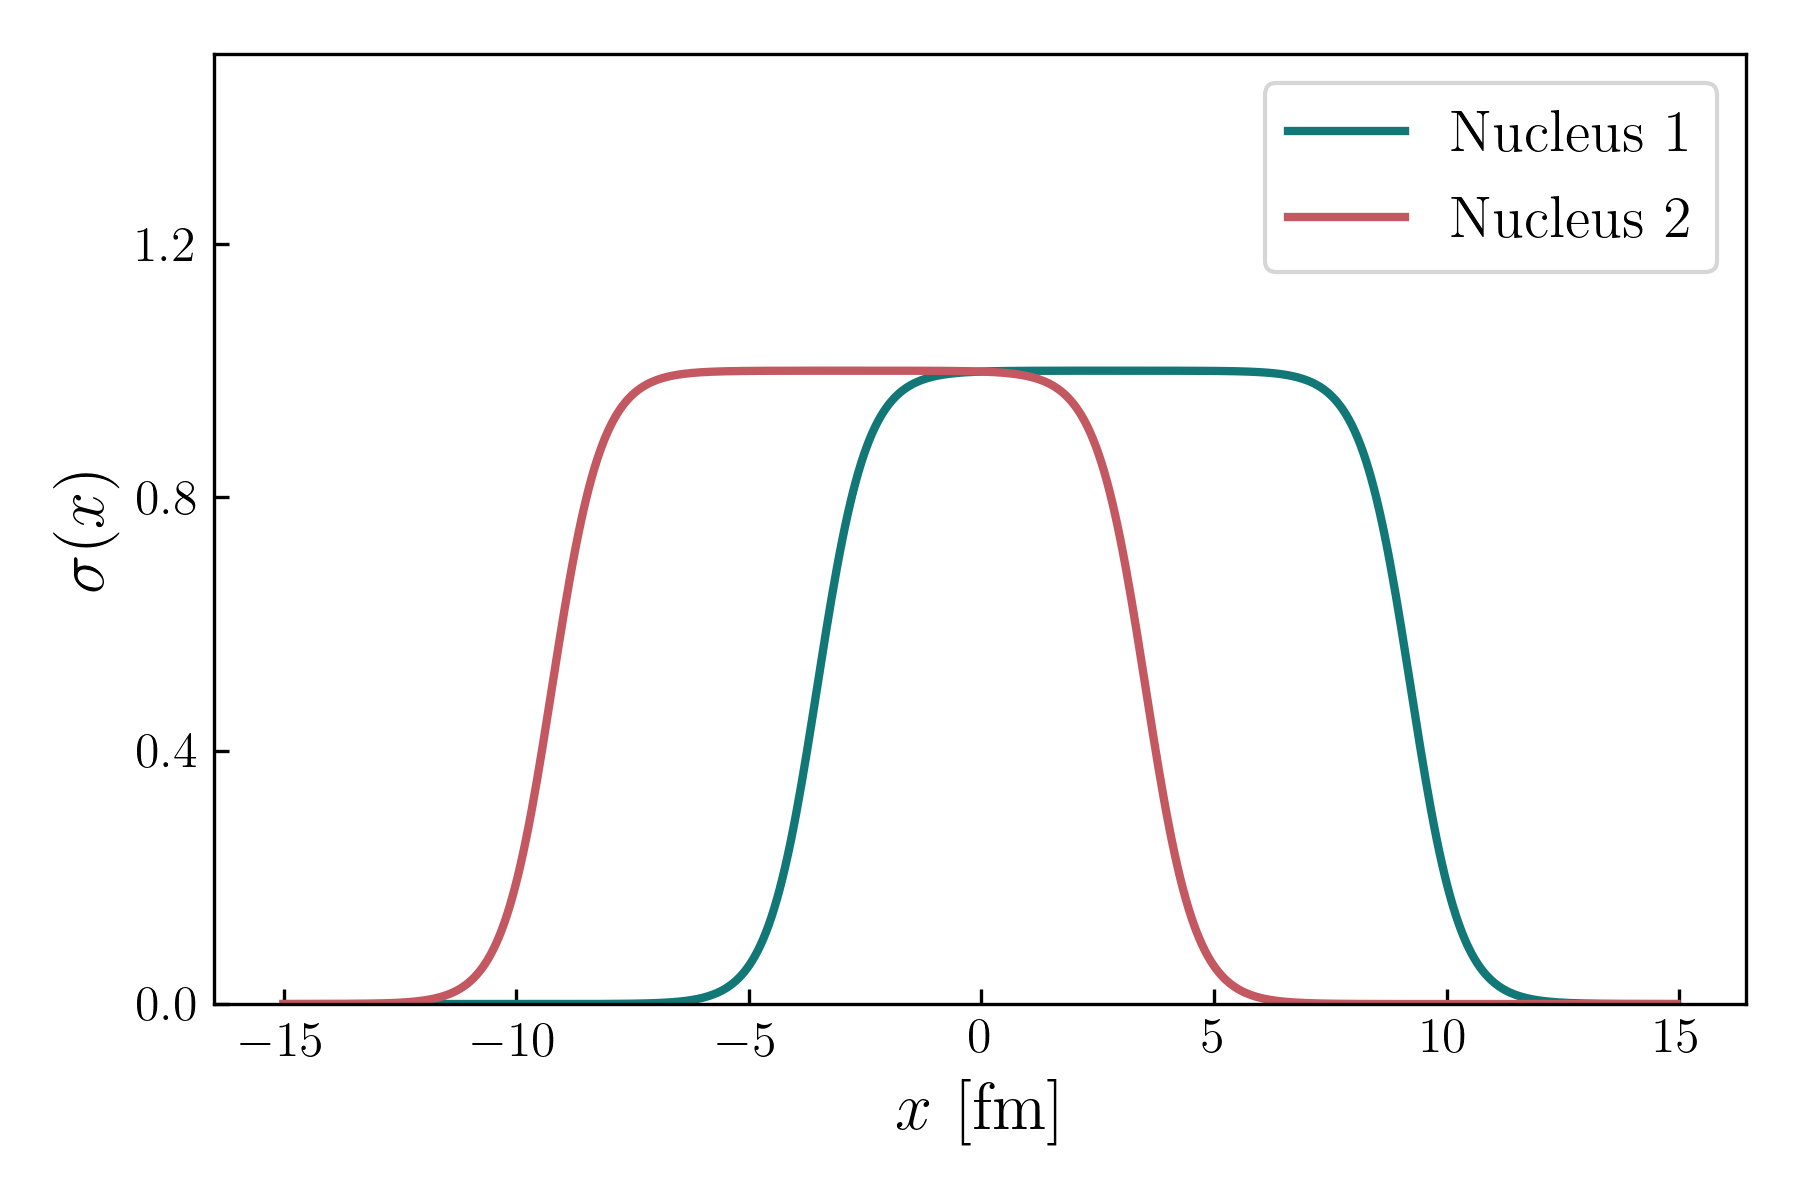
\includegraphics[width=\textwidth]{woods_saxon_auau_200.png}
	\caption{\normalsize Woods-Saxon distribution $\sigma(x,y)$ as a function of $x$ at $y=0$ for a $10$-$20\%$ centrality event having $b=5.7$ fm.} 
\end{figure}

Off-central collisions are thus obtained by shifting the transverse radius\sidenote{For example, with $b/2$ for nucleus $\textsf{1}$ and $-b/2$ for nucleus $\textsf{2}$.}with $\pm b/2$.

\begin{figure}[!hbt]
	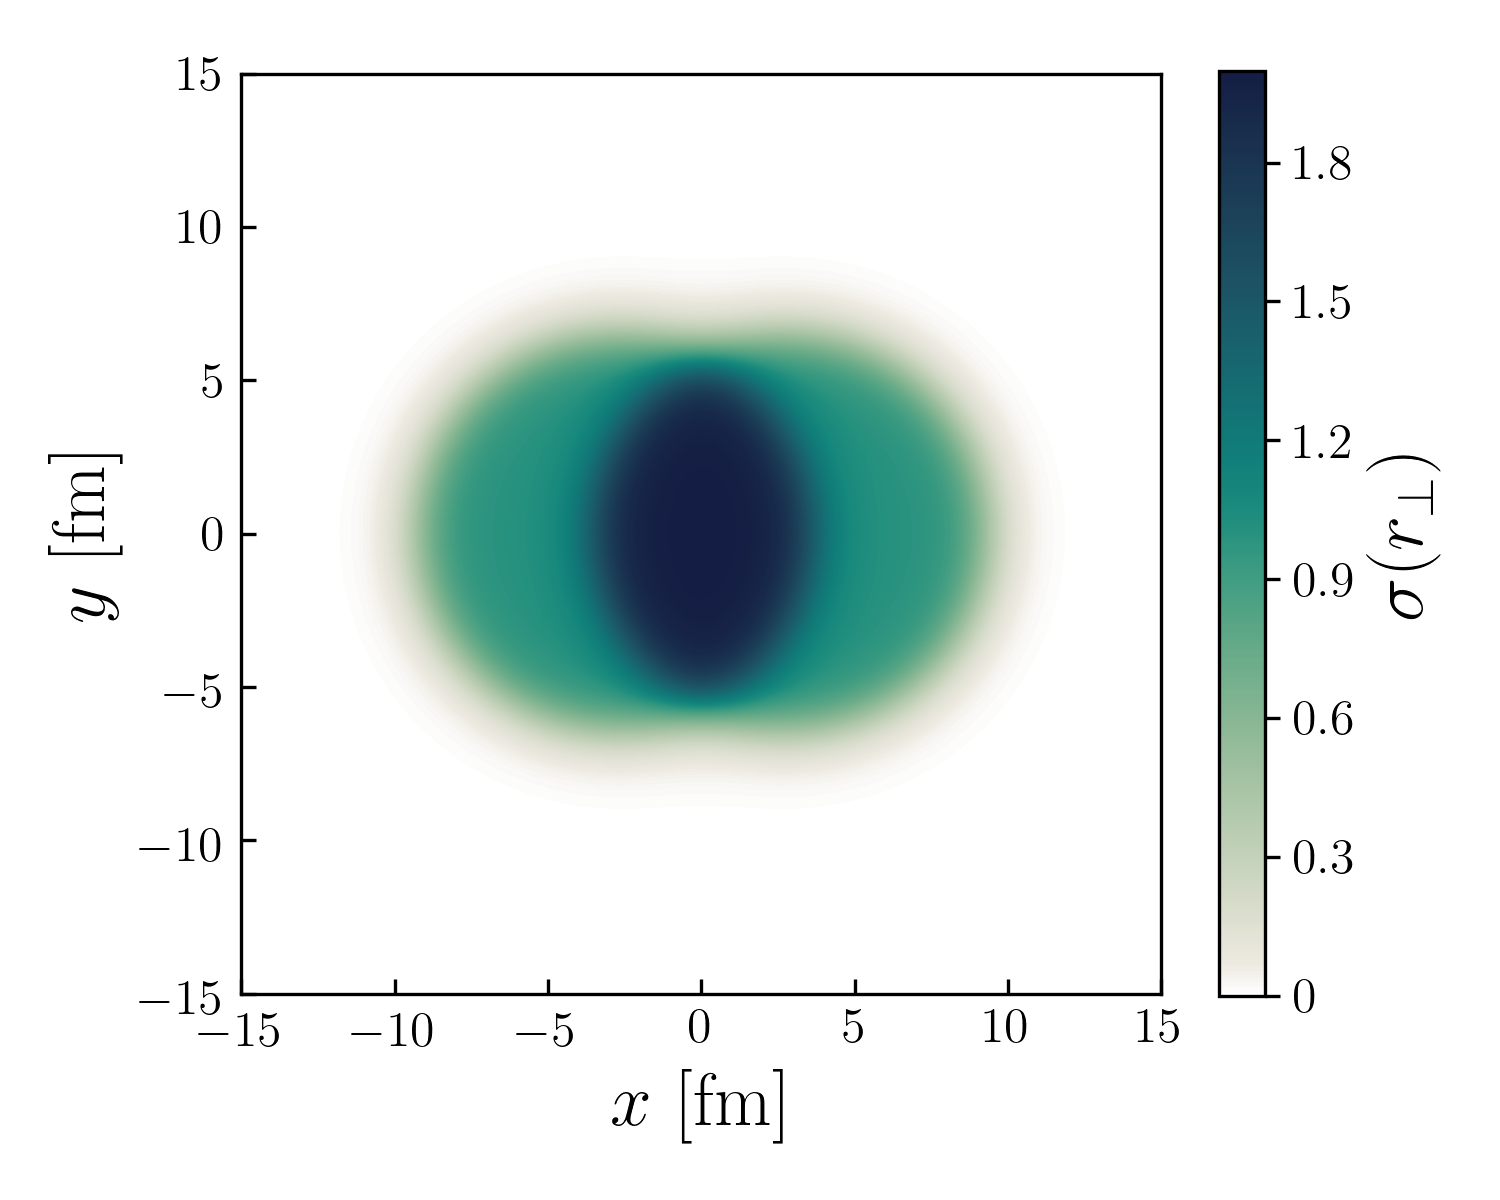
\includegraphics[width=0.833\textwidth]{woods_saxon_3d_auau_200.png}
	\caption{\normalsize Woods-Saxon distribution $\sigma(r_\perp)$ in the transverse plane $(x,y)$ for an event within $10$-$20\%$ centrality having $b=5.7$ fm.} 
\end{figure}


\subsubsection*{Landau matching}
The Glasma exhibits pressure anisotropy and within a classical description,\sidenote{Using non-Abelian Yang-Mills theory.}it may never reach isotropy. Nevertheless, the produced {\sffamily QGP} may very well be described by employing an ideal hydrodynamics evolution \cite{kolb, huovinen}, during which the medium is assumed to be isotropic. In order to match this distinct and irreconcilable scenarios, we are going to discard information from the Glasma energy-momentum tensor.\sidenote{By neglecting the components which would deviate the system from equilibrium.}One may construct an ideal energy-momentum tensor through a procedure named {\sffamily\color{ming} Landau matching} as\sidenote{Here $\textsf{P}$ represents the pressure and may be computed once an equation of state is provided, namely $\textsf{P}=\textsf{P}(\varepsilon,T)$.}
\begin{align*}
    \textsf{T}^{\mu \nu}=(\varepsilon_\textsf{LRL}+\textsf{P}) u^{\mu} u^{\nu}-\textsf{P} g^{\mu \nu}=\textsf{Diag}\{\varepsilon_\textsf{LRL}, \textsf{P}, \textsf{P}, \textsf{P}\},
\end{align*}
where the local rest frame ({\sffamily LRF}) energy density $\varepsilon_\textsf{LRL}$ and the flow velocity $u^\mu$ may be obtained by solving\sidenote{Where $T^{\mu\nu}$ is the energy-momentum tensor of the Glasma. One must only choose time-like flow vectors $u^\mu u_\mu=1$.}the eigenequation
\begin{align}\label{matt}
    T_{\nu}^{\mu} u^{\nu}=\varepsilon_\textsf{LRL} u^{\mu}.
\end{align}

\begin{figure*}[h!]
	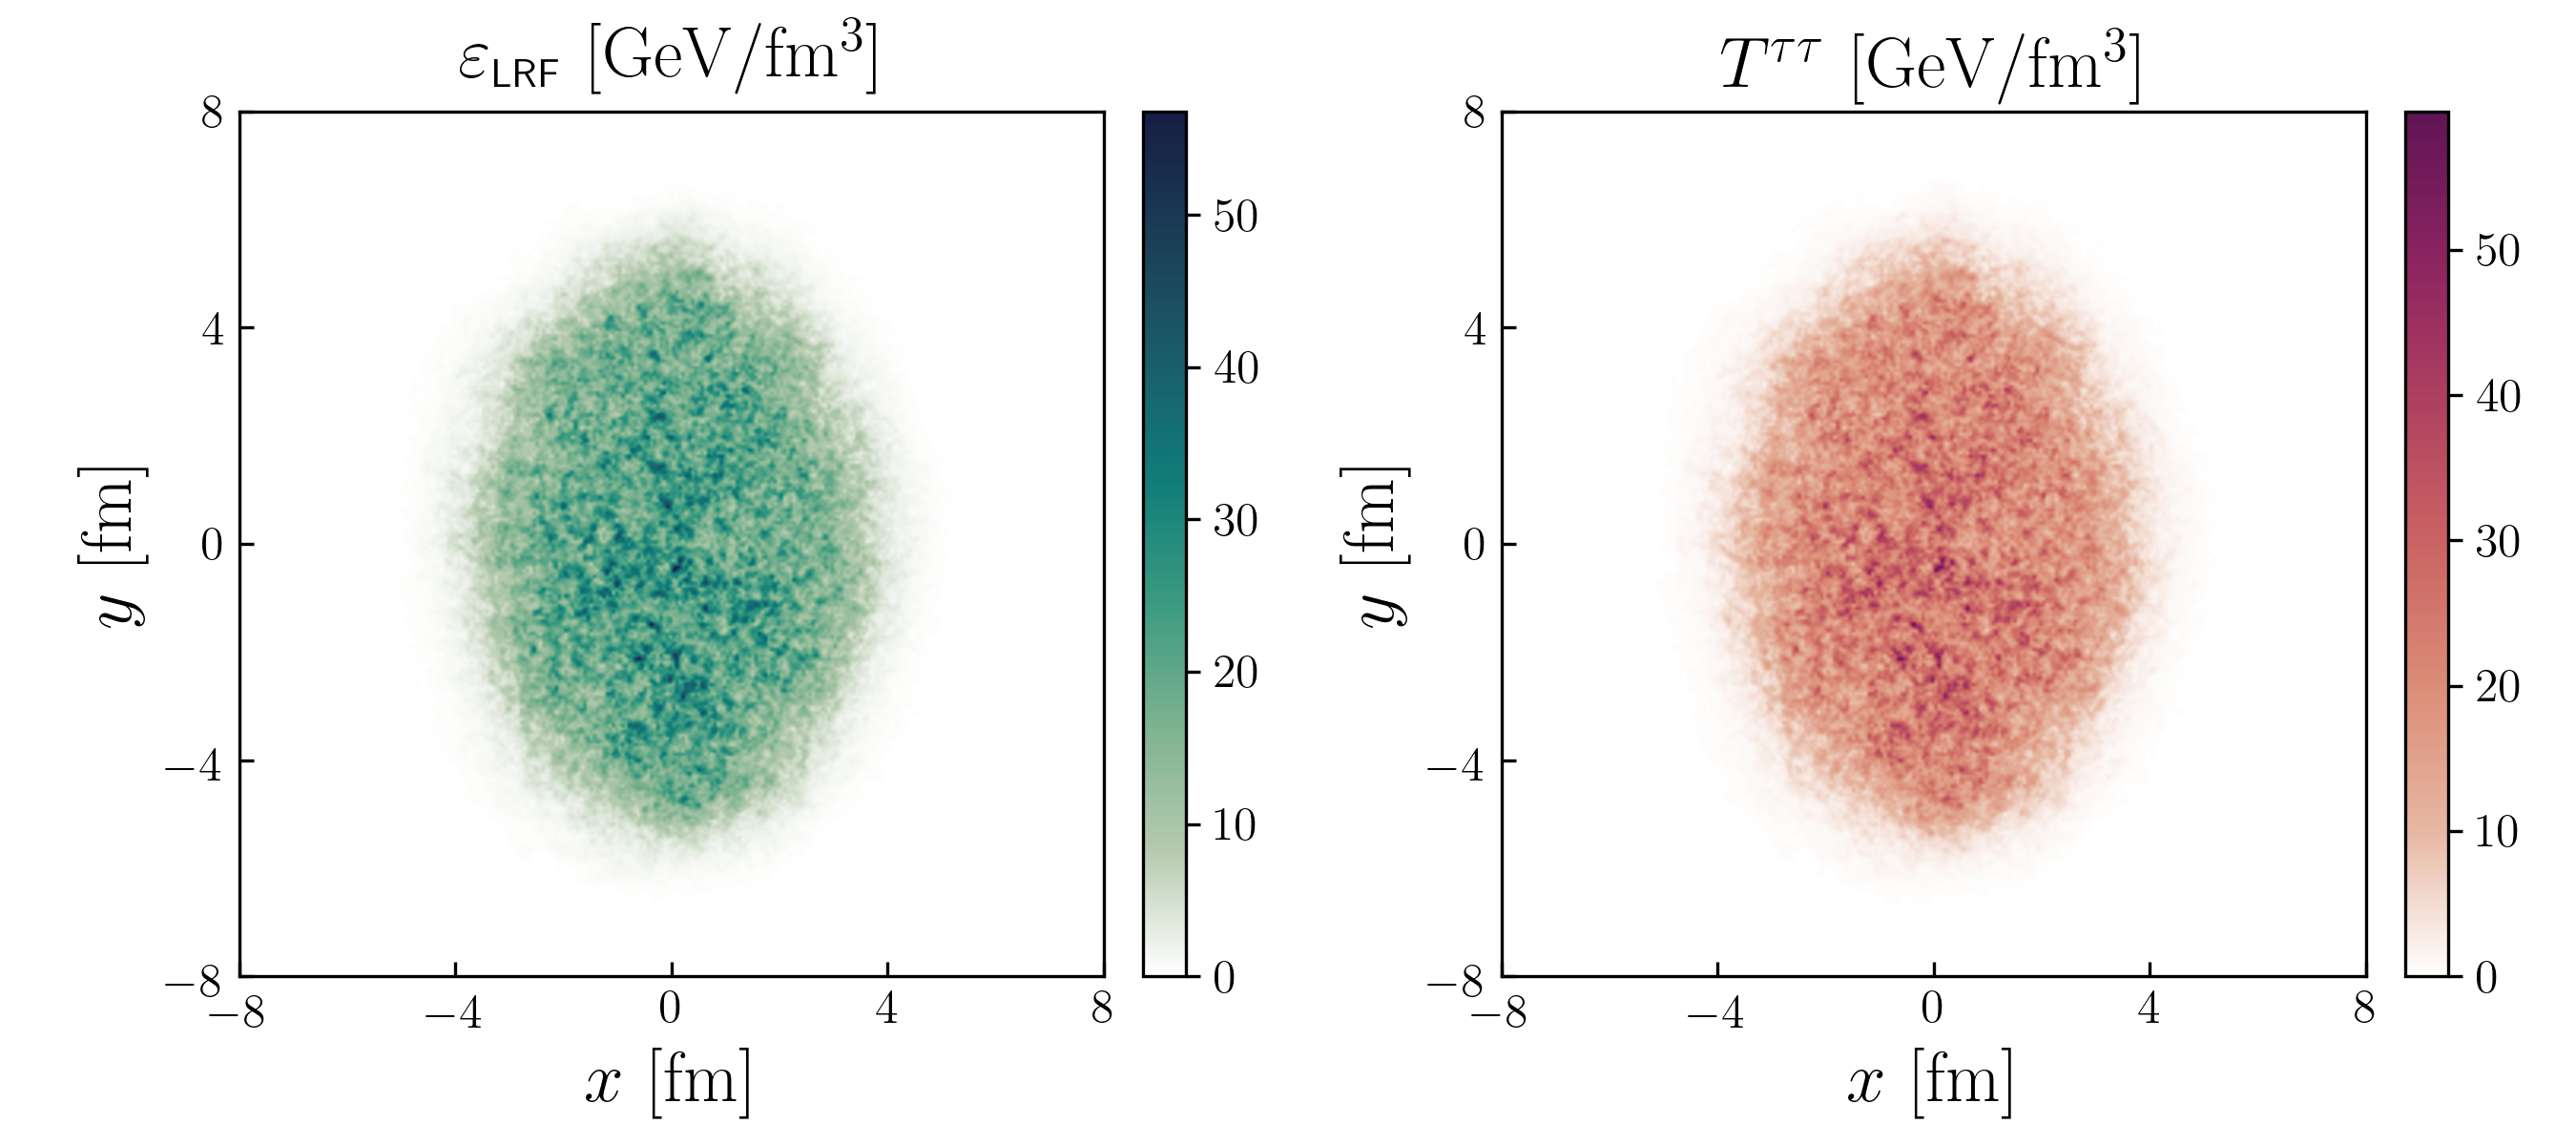
\includegraphics{images/ed_lrl_lab_auau_200_dpi_300.png}
	\caption{\normalsize Qualitative comparison between the local rest frame $\varepsilon_\textsf{LRL}$ and $T^{\tau\tau}$ component of the Glasma energy-momentum tensor, evaluated at $\tau_\mathrm{switch}=0.4$ fm/c for a $10$-$20\%$ centrality event with $b=5.7$ fm.}
\end{figure*}

\begin{note}
For a dissipative fluid which is near equilibrium, one may decompose the energy-momentum tensor as\sidenote{Once dissipation exhibits itself, thermodynamic quantities, which were well defined only for a fluid at local thermal equilibrium, may no longer be used.}
\begin{align*}
    T^{\mu\nu}=T^{\mu\nu}_\text{ideal}+\delta T^{\mu\nu}.
\end{align*}
Nevertheless, one may artificially assure local equilibrium by imposing the Landau matching condition\sidenote{Valid for an arbitrary $u^\mu$.}through
\begin{align*}
    u_\mu u_\nu \delta T^{\mu\nu}=0,
\end{align*}
which further yields\sidenote{In this way, the equilibrium component of $T^{\mu\nu}$ may be constructed from the local rest frame energy $\varepsilon_\textsf{LRL}$.}
\begin{align*}
    \varepsilon_\textsf{LRL}=u_\mu u_\nu T^{\mu\nu}.
\end{align*}
For a dissipative system in which both energy and particle diffusion coexist, one may define the {\sffamily LRL}\sidenote{For the ideal fluid, a {\sffamily LRF} was simply the frame in which the fluid volume element was at rest and both the energy and particle flows were null.}in multiple ways. Nevertheless, there exist two simple choices: the Eckart frame, where the energy flow is null, and the Landau frame, in which particle flow vanishes.\sidenote{This choice is more appropriate for ultrarelativistic heavy-ion collisions since they take place at negligible net baryon current.}In the Landau frame, the flow velocity $u^\mu$ is chosen to be along the energy flow velocity $T^{\mu\nu}u_\nu$, that is
\begin{align*}
    u_\nu T^{\mu\nu}=\varepsilon_\textsf{LRL}u^\mu.
\end{align*}
\end{note}

In the boost-invariant approximation, one may further neglect the longitudinal flow component\sidenote{As emphasized in \cite{mcdonald} and showed in \cite{mcdolandflow}, this component turns out to also be of relevance.}$u^\eta=0$. Hence, the problem reduces to finding the eigenvalues $\varepsilon_\textsf{LRL}$ and eigenvectors $(u^\tau, u^x, u^y)$ of a $3\times 3$ sub-matrix of $T^{\mu\nu}$. 

One may define flow velocities weighted with respect to the energy density as\sidenote{Where $w^\perp\overset{\Delta}{=}(w^x,w^y)$ and similarly for $u^\perp$.}
\begin{align*}
    w^\perp\overset{\Delta}{=}\dfrac{\varepsilon_\textsf{LRL}}{\langle\varepsilon_\textsf{LRL}\rangle}u^\perp.
\end{align*}

\vspace{-0.5cm}

\begin{figure*}[h!]
	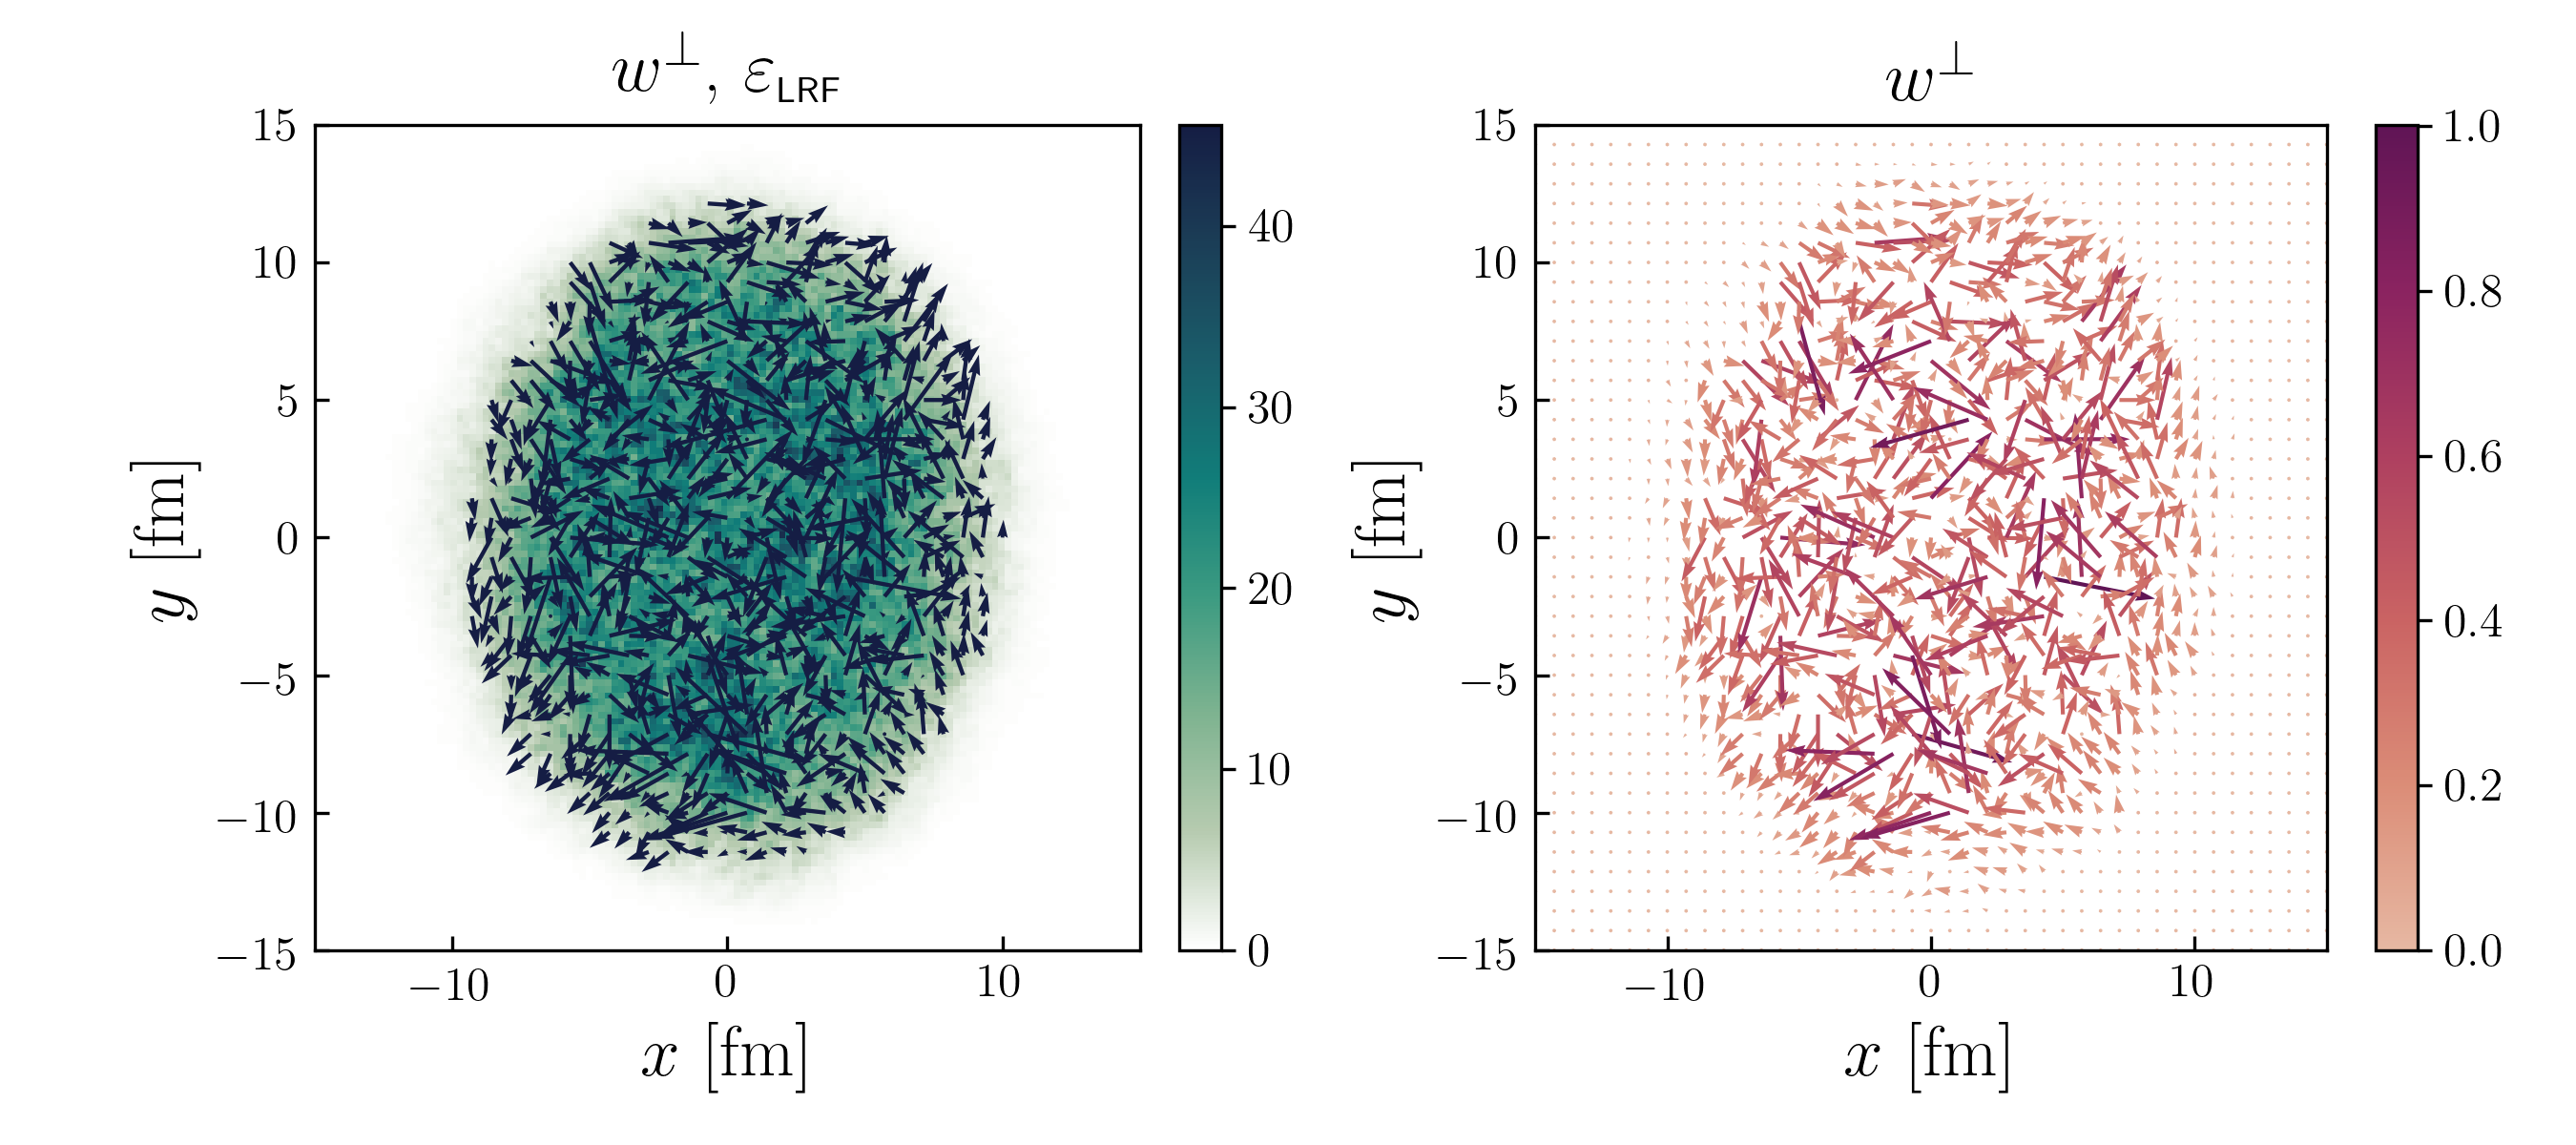
\includegraphics{images/ed_u_auau_200_dpi_300.png}
	\caption{\normalsize Weighted flow velocity $w^\perp$ superimposed over the local rest frame $\varepsilon_\textsf{LRL}$, evaluated at $\tau_\mathrm{switch}=0.4$ fm/c for a $5$-$10\%$ centrality event with $b=3.7$ fm.}
\end{figure*}

\begin{figure}[!hbt]
	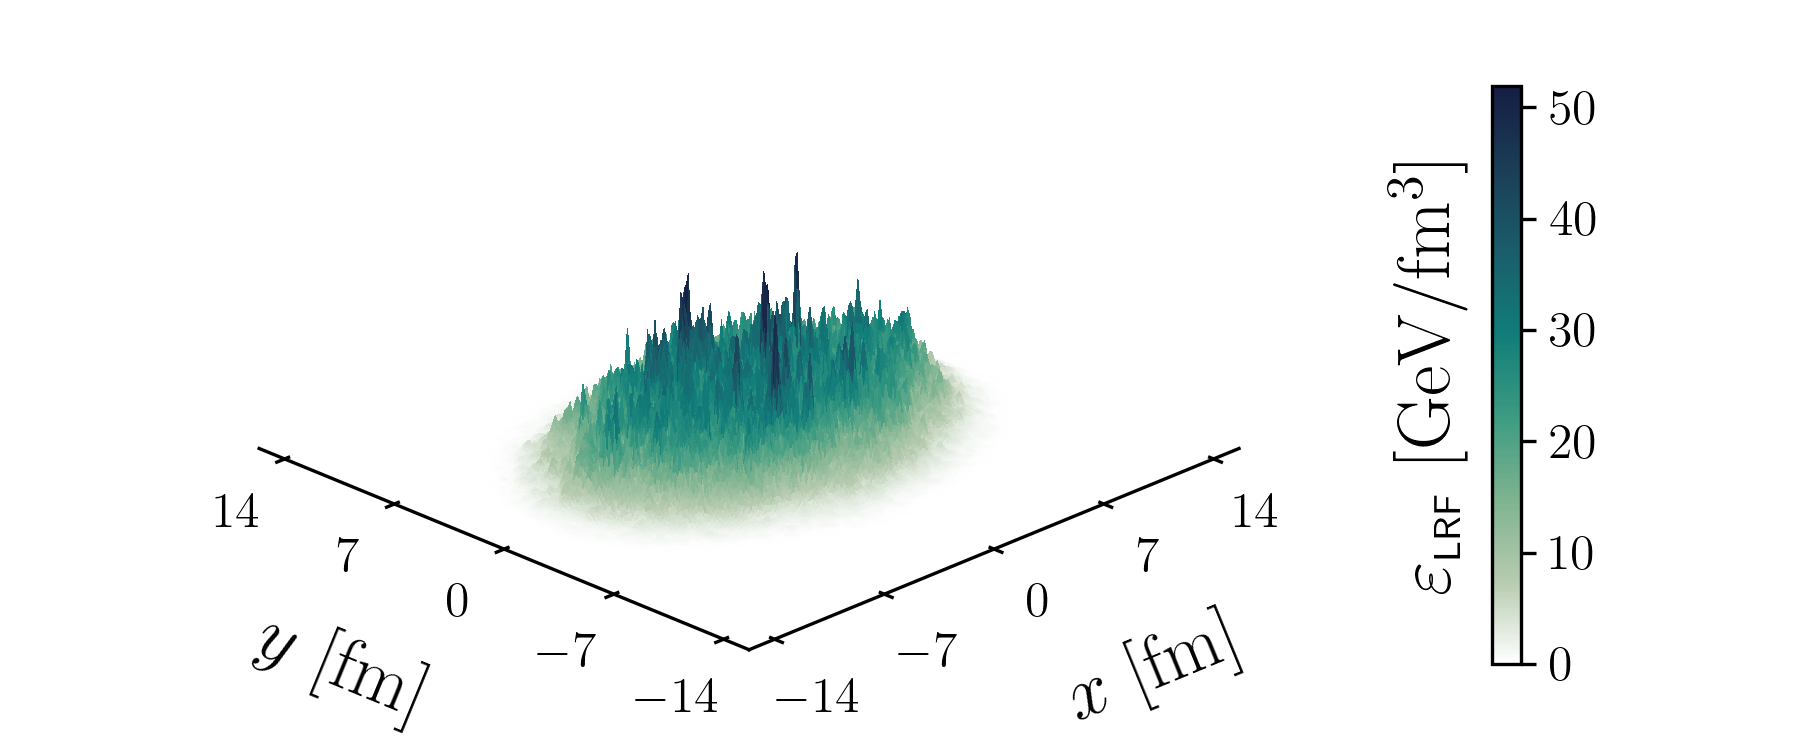
\includegraphics[trim=40 0 40 0,clip,width=\textwidth]{ed_3d.png}
	\caption{\normalsize Energy density in the local rest frame $\varepsilon_\textsf{LRL}$ as a function of the transverse coordinates, evaluated at $\tau_\mathrm{switch}=0.4$ fm/c for a $10$-$20\%$ centrality event with $b=5.7$ fm. One may notice spikes arising from the highly dense regions of the Glasma.} 
\end{figure}

\section{Centrality selection}
Each event requires an impact parameter as input. In order to mimic the minimum bias centrality selection, one needs to simulate many events\sidenote{We simulated $5\cdot 10^{4}$ events.}with impact parameters\sidenote{In the range $b\in(0,3r_0)$, that is $b\approx 0\divisionsymbol 18$ fm.}randomly distributed according to
\begin{align*}
    \textsf{P}(b)db=\dfrac{bdb}{b^2_\text{max}/2}.
\end{align*}
The centrality selection should be performed in terms of the final charged particle multiplicity $dN_\text{ch}/d\eta$ but we are going to apply the centrality cuts before the hydrodynamic evolution\sidenote{We are going to make use of the fact that there exists a good correlation between the initial energy in the central pseudorapidity region and the final charged multiplicity.}since performing hydrodynamics simulations on such a large number of events is computationally expensive and time consuming. \\
The Glasma fields are evolved until $\tau_\text{swith}=0.4$ fm/c. We already observed that for proper times $\tau>0.1$ fm/c the expansion of the system is of Bjorken type. Hence, the energy density at mid-pseudorapidity of the Glasma may be expressed as \cite{bjorken}
\begin{align*}
    \varepsilon(\tau)\approx \frac{1}{\textsf{S}_\perp}\left(\frac{1}{\tau}\frac{dE_\perp}{d\eta}\right).
\end{align*}

\vspace{-0.5cm}

\begin{figure*}[h!]\labfig{centralitycut}
	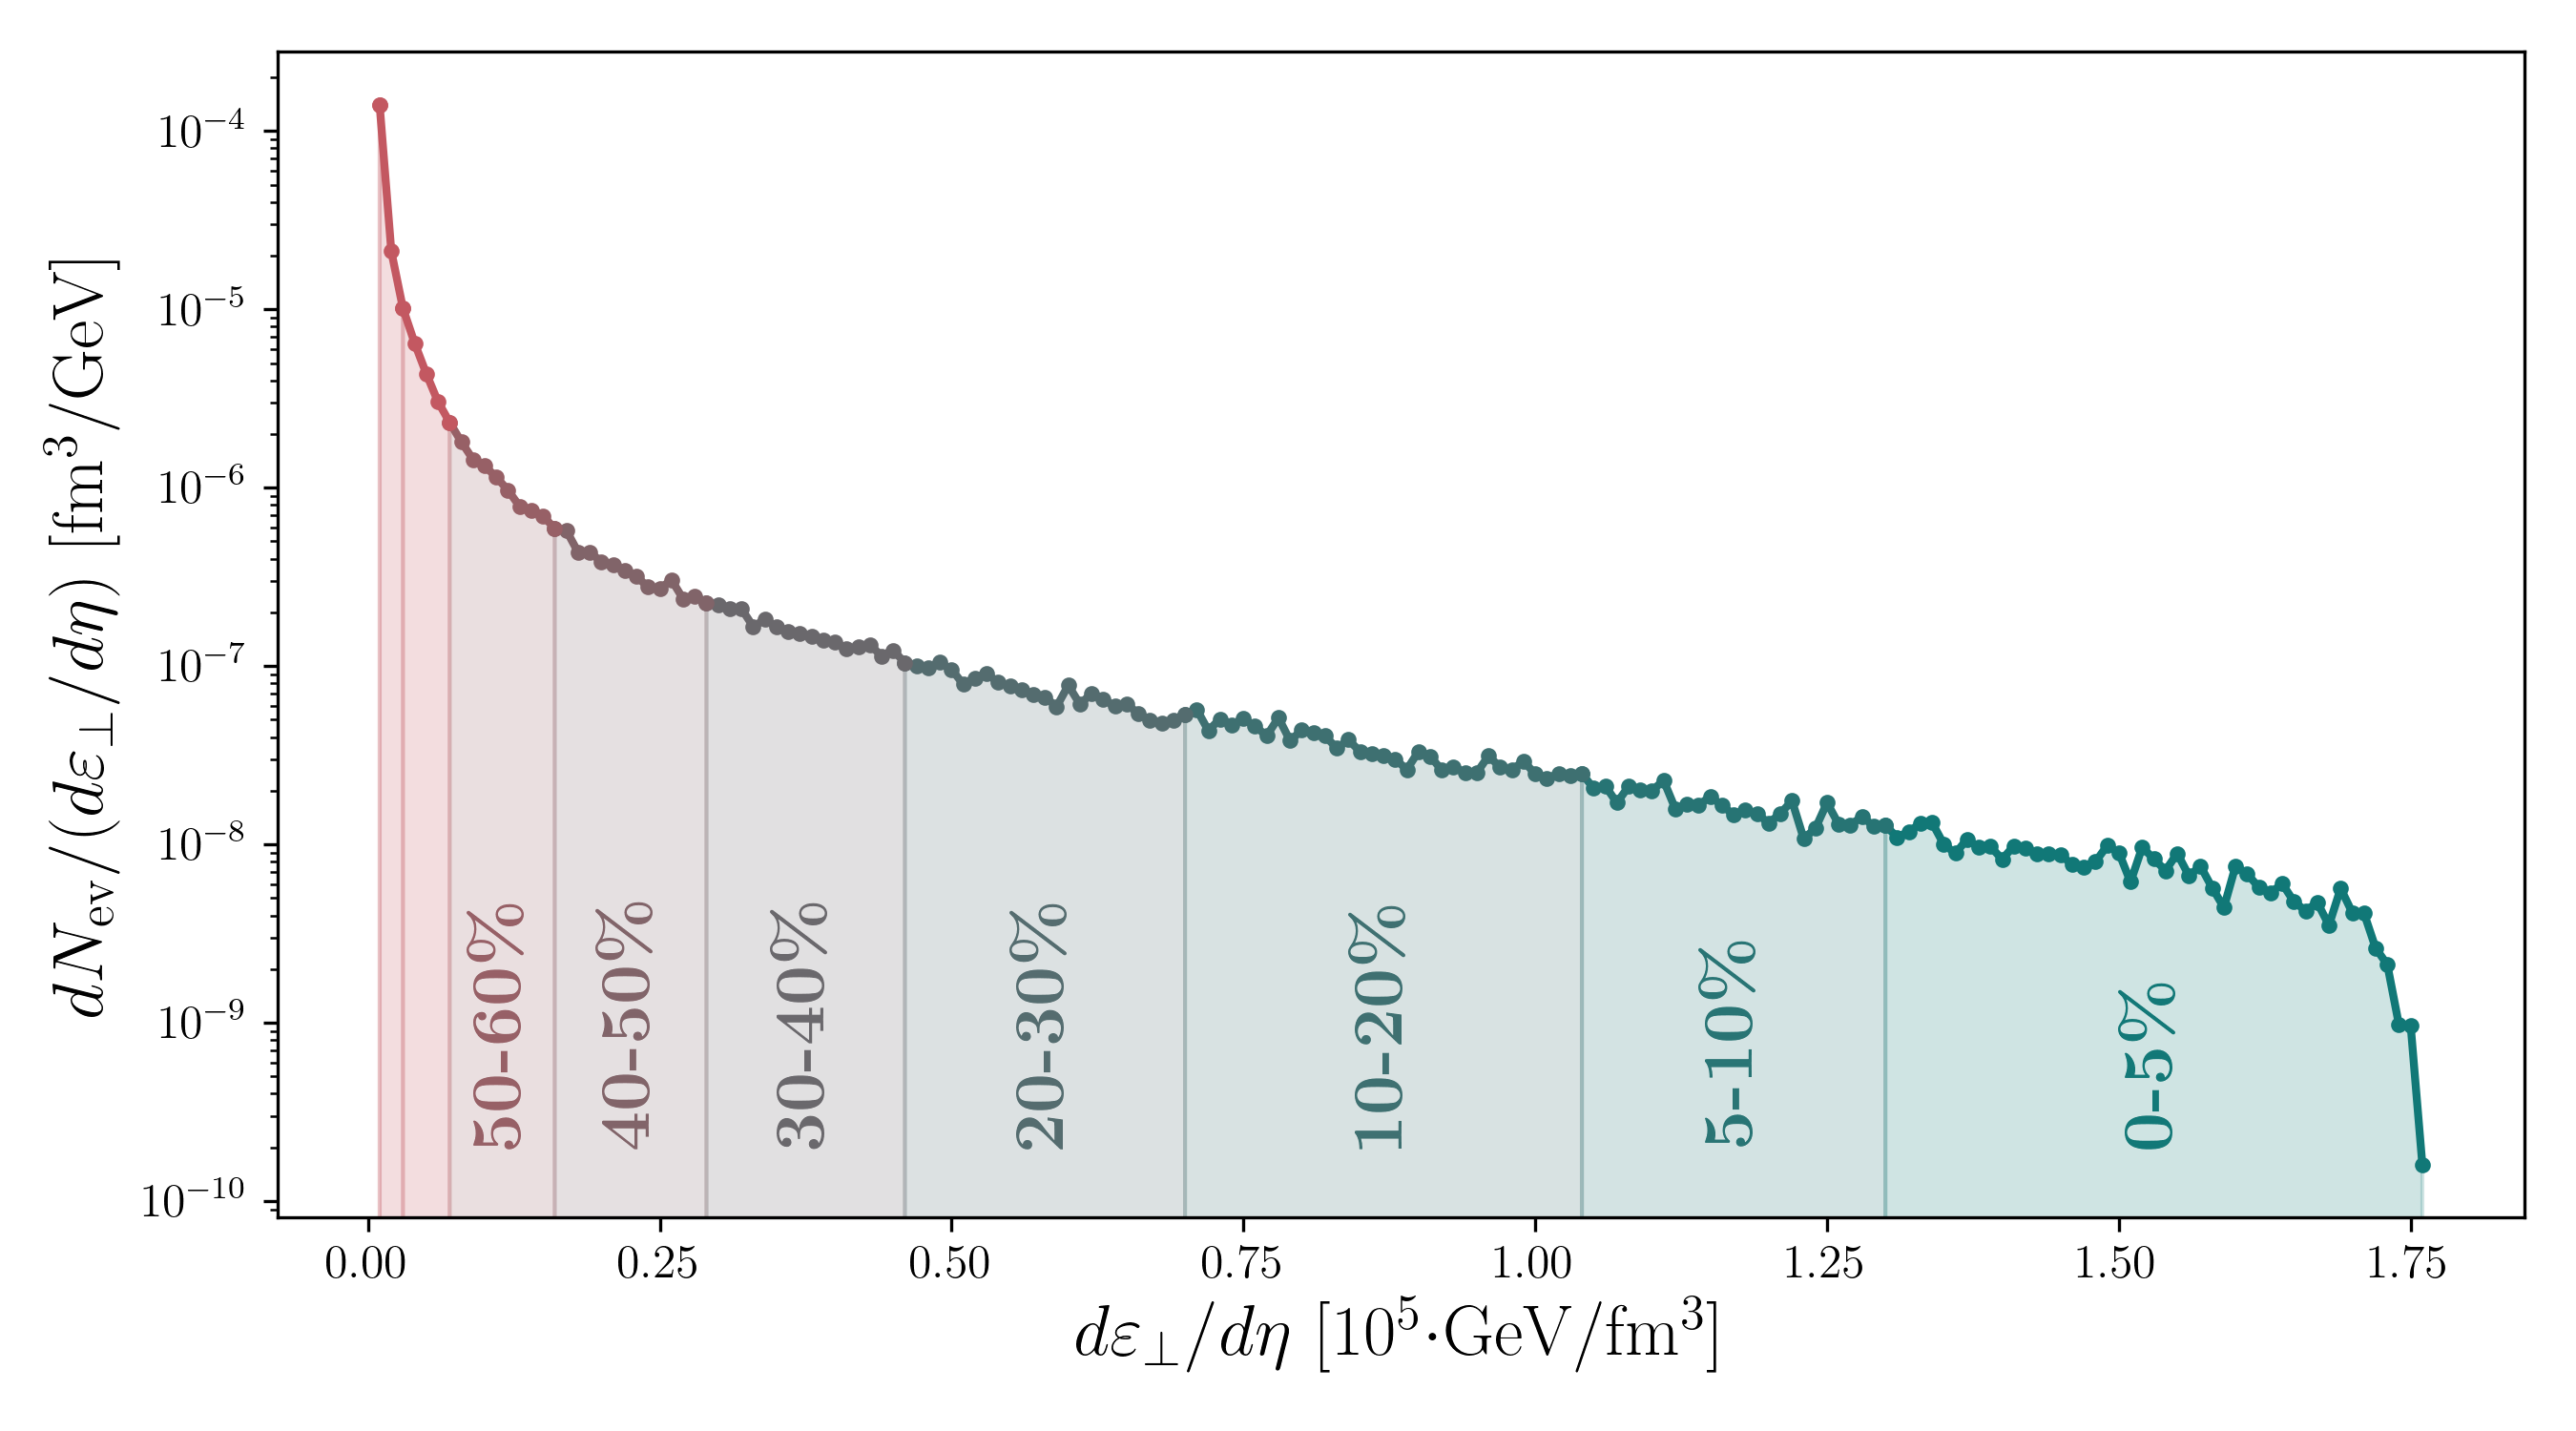
\includegraphics{images/centrality_cut.png}
	\caption{\normalsize Minimum bias centrality selection using $5\cdot 10^4$ events simulated with {\sffamily Curraun}, divided in centrality classes according to their total energy density in the transverse plane $d\varepsilon_\perp/d\eta$.}
\end{figure*}

Therefore, we shall split the events resulting from {\sffamily Curraun} in terms of the total energy density\sidenote{It's not possible to directly evaluate the overlapping area in the transverse plane $\textsf{S}_\perp$ but one may numerically extract
\begin{align*}
    \frac{1}{\tau}\frac{dE_\perp}{d\eta}\Bigg|_{\tau}=(a_T)^2\frac{d\varepsilon_\perp}{d\eta}\Bigg|_{\tau},
\end{align*}
evaluated at $\tau=0.4$ fm/c, where $d\varepsilon_\perp/d\eta$ is the total energy density in the transverse plane.}$d\varepsilon_\perp/d\eta$. Nevertheless, such an approach turns out to be problematic since, within a model constructed with fields, one may not provide a clear criteria whether a collision event occurs or not. \\

Thus, the $100\%$ centrality cut must be chosen by hand. We shall attempt to guess it though an iterative procedure. Since $d\varepsilon_\perp/d\eta$ is correlated with $dN_\text{ch}/d\eta$, one may vary this cut until the ratios between the total energy density in different centrality cuts match the corresponding experimental multiplicity ratios. A later scaling of the energy density should not affect this centrality selection. It is important to mention that\sidenote{Since the previously mentioned correlation is only approximate.}some events may end up in a different centrality class after the hydrodynamic evolution.

\begin{figure}[!hbt]
	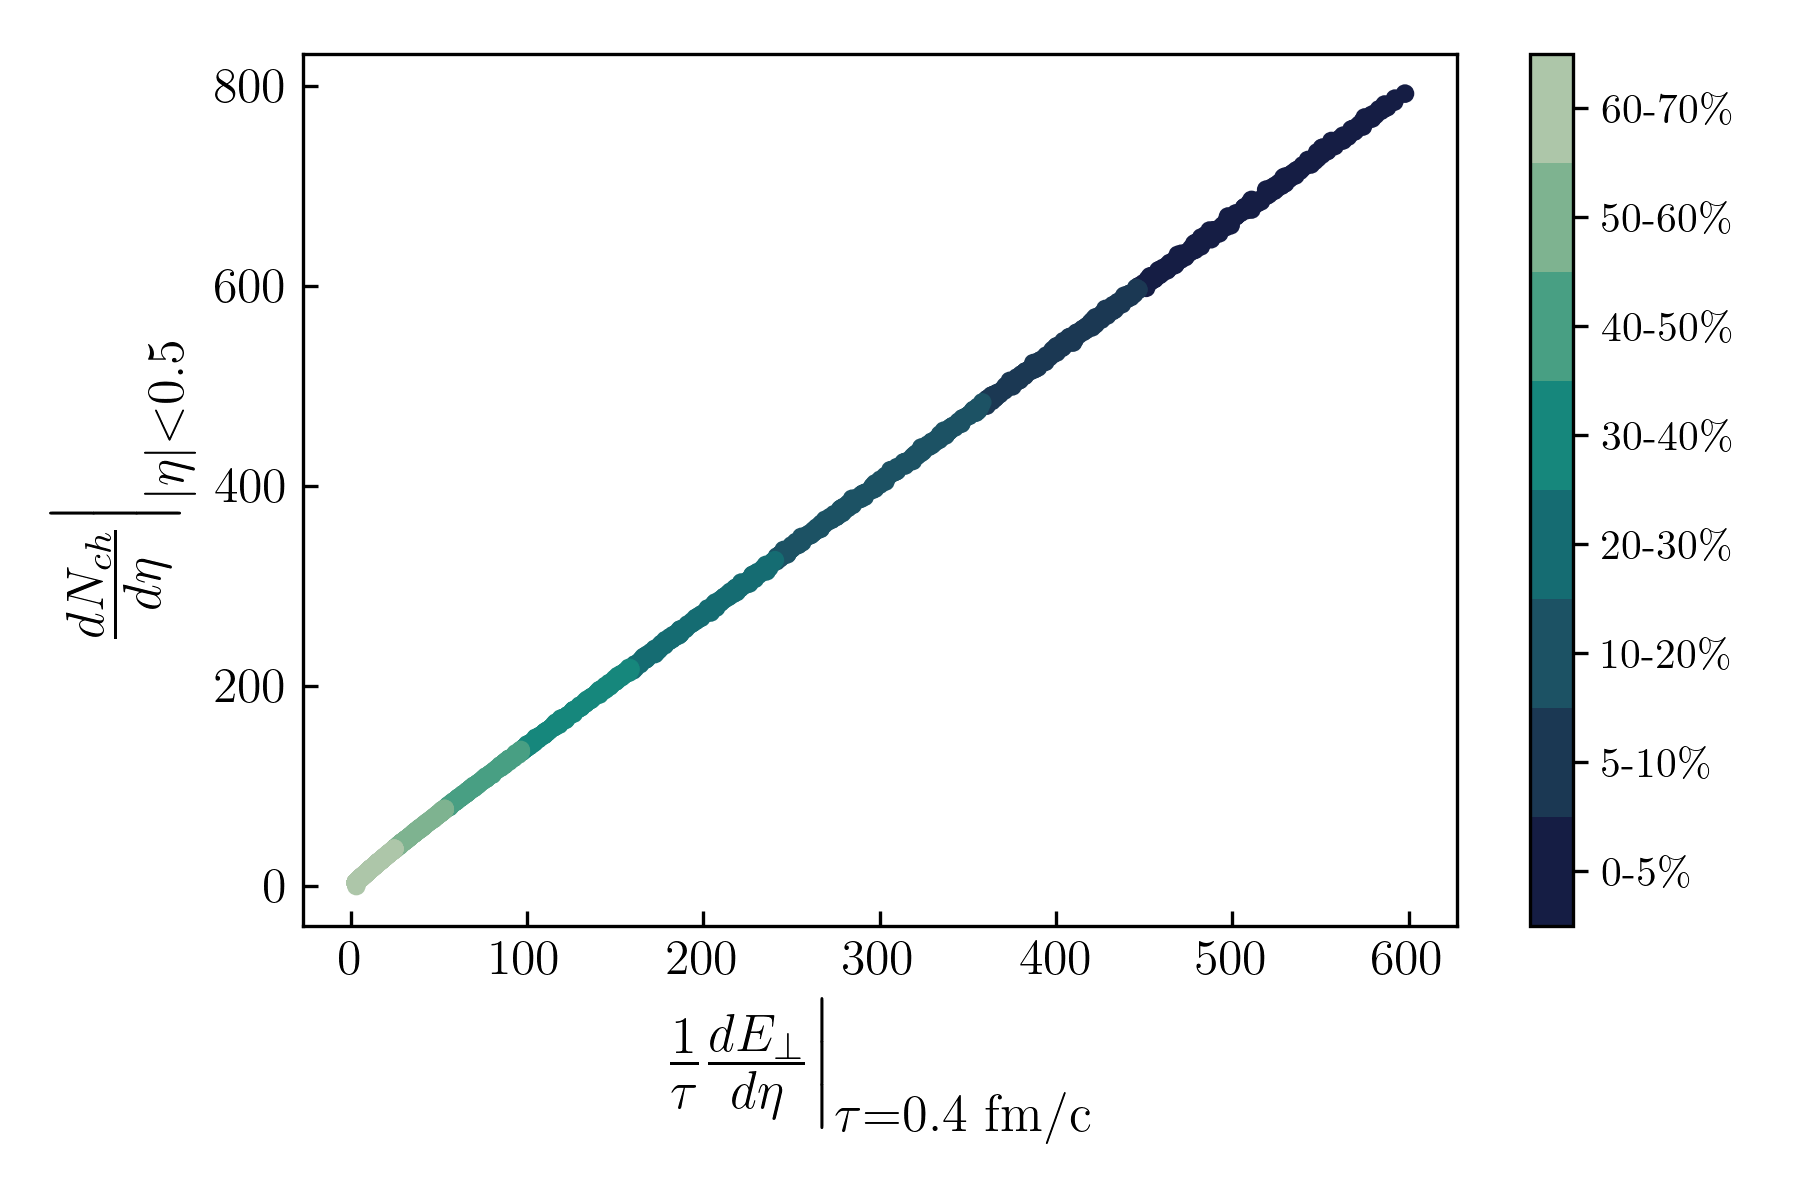
\includegraphics[width=\textwidth]{images/dnch_etot.png}
	\caption{\normalsize Correlation between the initial $d\varepsilon_\perp/d\eta$ and the final $dN_\mathrm{ch}/d\eta$ for a subset of $2700$ events with $300$ events per centrality. Main simulation parameters: $\eta/s=0.24$ and $T_\mathrm{fo}=180$ MeV. A power law fit yields
	\begin{align*}
	    \frac{dN_\text{ch}}{d\eta}\approx 2.1 \left(\frac{1}{\tau}\frac{dE_\perp}{d\eta}\right)^{0.93}.
	\end{align*}
	} 
\end{figure}

\begin{figure}[!hbt]
    \figcolor{tealblue}
	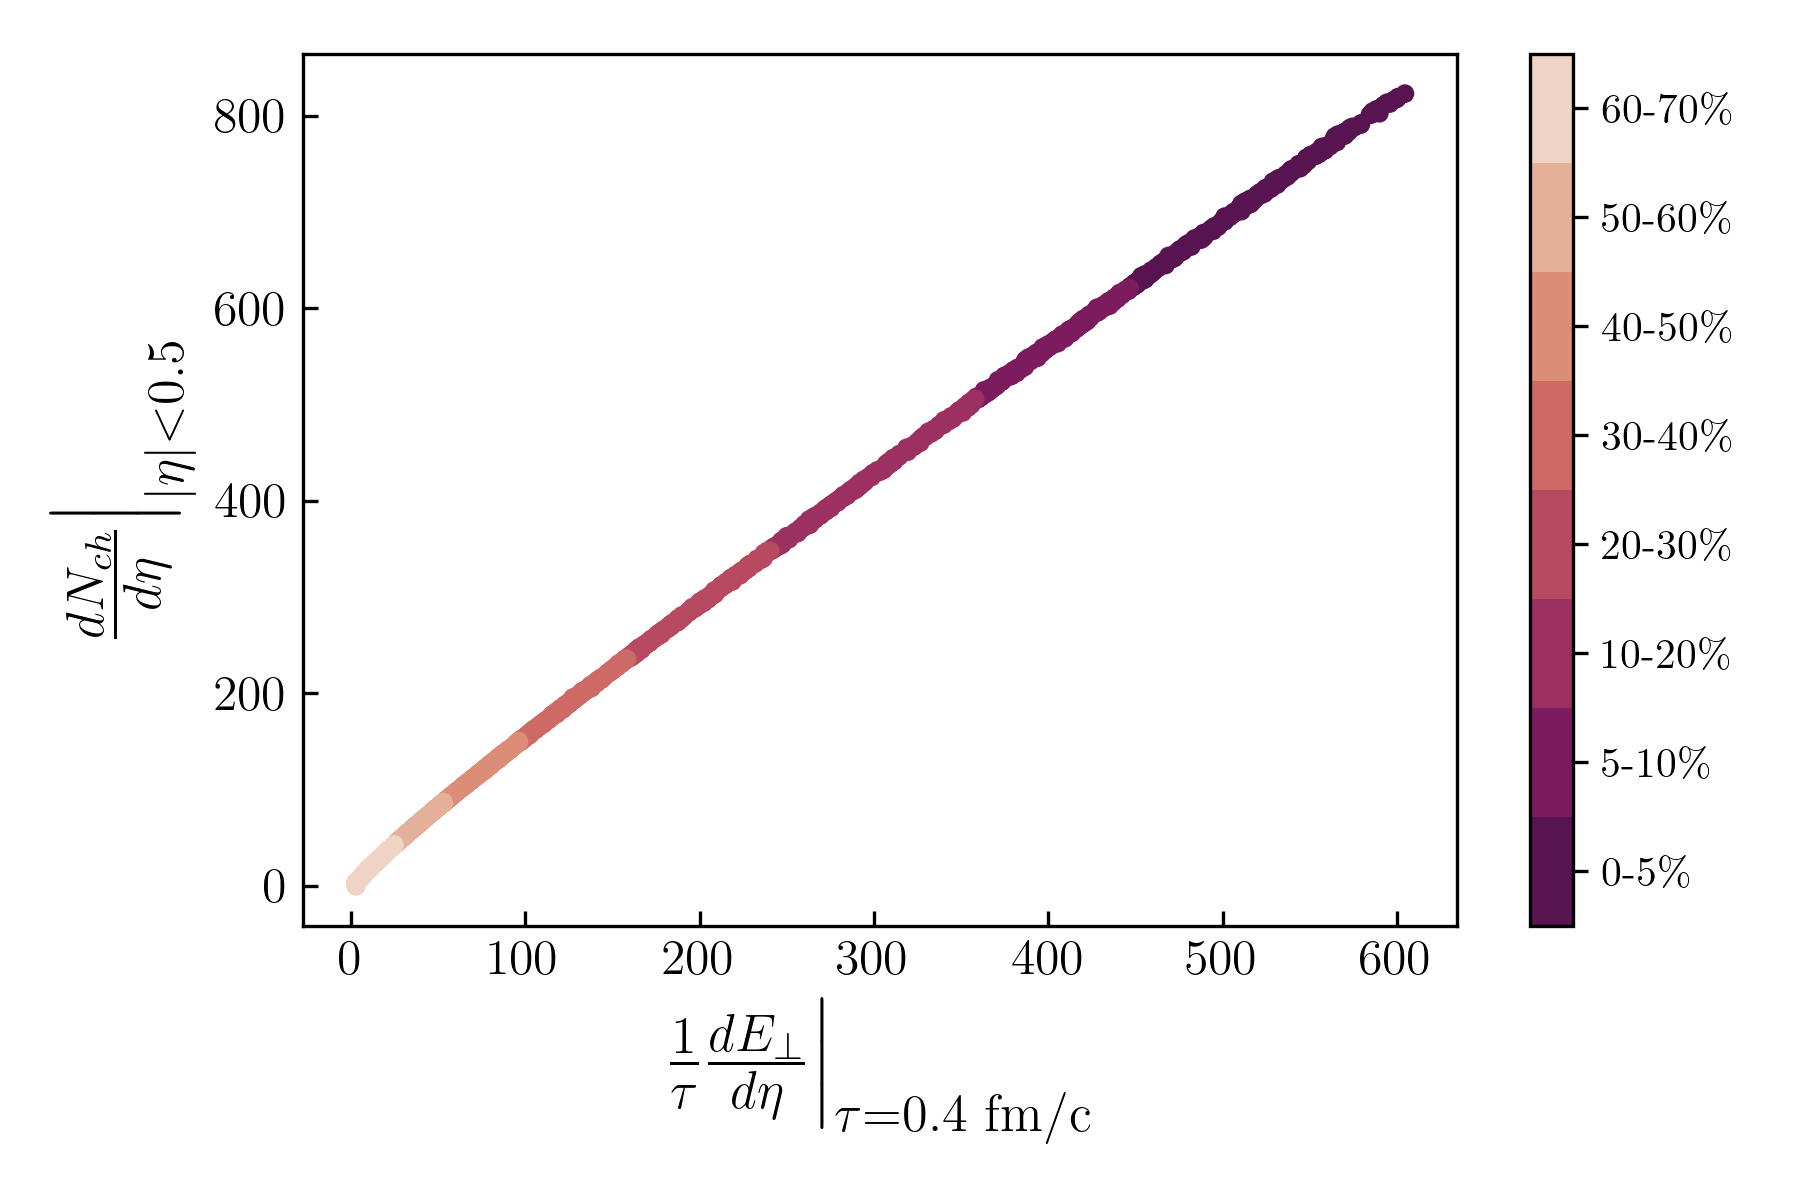
\includegraphics[width=\textwidth]{images/dnch_etot_bulk.png}
	\caption{\normalsize Correlation between the initial $d\varepsilon_\perp/d\eta$ and the final $dN_\mathrm{ch}/d\eta$ for a subset of $2700$ events with $300$ events per centrality. Main simulation parameters: $\eta/s=0.1$ and $T_\mathrm{fo}=180$ MeV and hard-coded $\zeta(T)$. A power law fit yields
	\begin{align*}
	    \frac{dN_\text{ch}}{d\eta}\approx 1.56 \left(\frac{1}{\tau}\frac{dE_\perp}{d\eta}\right)^{0.96}.
	\end{align*}
	} 
\end{figure}

An alternative approach \cite{mcdonaldhydro} would be to take a subset from the total events, pass them trough the hydrodynamic simulation, extract the final multiplicities and then map\sidenote{And obtain a parametrization of the type
\begin{align*}
    \frac{dN_\text{ch}}{d\eta}=\mathrm{const}\left(\frac{1}{\tau}\frac{dE_\perp}{d\eta}\right)^\text{power}.
\end{align*}
}$dN_\text{ch}/d\eta$ as a function of $d\varepsilon_\perp/d\eta$. Afterwards, one may perform a centrality selection using this map. The disadvantage would be that such a map and hence the centrality selection depends on the parameters from the hydrodynamic simulation. 

\section{Relativistic viscous hydrodynamics}
\subsubsection{Viscous hydrodynamics primer}
Starting from the energy-momentum tensor for the ideal fluid\sidenote{Where $\Delta^{\mu\nu}$ acts as a projector operator onto the space perpendicular to $u^\mu$. This may be inferred from its properties, namely $\Delta^{\mu\nu}u_\mu=\Delta^{\mu\nu}u_\nu=0$ and $\Delta^{\mu\nu}\Delta^\alpha_\nu=\Delta^{\mu\alpha}$.}
\begin{align*}
    T^{\mu\nu}_\text{eq}=\varepsilon u^\mu u^\nu-\textsf{P}\Delta^{\mu\nu},
\end{align*}
one may add dissipative corrections\sidenote{This form is only valid in the Landau frame $T^{\mu\nu}u_\nu=\varepsilon u^\mu$.}
\begin{align*}
    T^{\mu\nu}=T^{\mu\nu}_\text{eq}-\Pi\Delta^{\mu\nu}+\pi^{\mu\nu}.
\end{align*}
Since the conservation of the energy momentum tensor\sidenote{This should be accompanied by the conservation of the charge current but we shall work with null baryon current.}
\begin{align*}
    \partial_\mu T^{\mu\nu}=0,
\end{align*}
along with an equation of state $\textsf{P}=\textsf{P}(\varepsilon,T)$ provide $4+1=5$ equations for a system with $1+1+3+1+5=11$ unknowns, additional information is needed to construct the viscous corrections.\\

One may attempt to use a relativistic version of the Navier-Stokes equations\sidenote{Which would result in 
\begin{align*}
    &\Pi=-\zeta\partial_\mu u^\mu,\\
    &\pi^{\mu\nu}=2\eta\nabla^{\langle\mu}u^{\nu\rangle},
\end{align*}
with $\zeta$ and $\eta$ being transport coefficients. More details in \cite{Jaiswal:2014lsa}.}but such an equation suffers from acausality: adding a small perturbation of energy density and flow velocity gives a parabolic dispersion relation and thus faster than light propagation. A solution is provided within the Israel-Stewart\sidenote{See \cite{Song:2009gc} for a more in depth review.}formulation by either using the second law of hydrodynamics\sidenote{Adding deviations from equilibrium to the entropy current.}or using kinetic theory.\sidenote{Considering small deviations from the equilibrium Boltzmann equation.} \\

In kinetic theory, all information is encoded in the microscopic distribution function $f(t,\vec{x},\vec{p})$. Within the Boltzmann approximation, it satisfies the equation
\begin{align*}
    p^{\mu} \partial_{\mu} f(t,\vec{x},\vec{p})=\mathcal{C}[f(t,\vec{x},\vec{p})],
\end{align*}
where $\mathcal{C}[f]$ represents the collision integral. One may construct the macroscopic energy-momentum tensor as
\begin{align*}
    T^{\mu \nu}(t, \vec{x}, \vec{p})=\sum\limits_ig_i \int \frac{d^{3} \vec{p}}{(2 \pi)^{3} E_{\vec{p}}} p^{\mu} p^{\nu} f_{i}(t, \vec{x}, \vec{p}),
\end{align*}
with $g_i$ denoting the degeneracy of the species $i$. \\
Dissipation may be added by considering small deviations of the distribution function $f=f_\text{eq}+\delta f$, with the equilibrium distribution given by\sidenote{That is Bose-Einstein or Fermi-Dirac distributions.} 
\begin{align*}
    f_\text{eq}(x, \vec{p})=\dfrac{1}{\exp{\dfrac{p \cdot u}{T}} \mp 1}.
\end{align*}
Further, one may deduce an evolution equation for $\delta f$ which, by making use of the energy-momentum conservation, leads to a set of equations for $\Pi$ and $\pi^{\mu\nu}$. They will turn out to depend on the collision kernel. Nevertheless, by employing Grad's $14$ momentum approximation\sidenote{In which the dissipative corrections are expanded up to quadratic terms in momentum.}
\begin{align*}
    \delta f(\vec{p})=f_\text{eq}(\vec{p})\left[A_0+A_{1}(p \cdot u)+A_2(p \cdot u)^{2}\right] \Pi+B_{0} \pi_{\mu \nu} p^{\mu} p^{\nu},
\end{align*}
they may be reduced to a closed form\sidenote{See \cite{ryu} for complete computations.}
\begin{fullwidth}
\begin{equation*}
    \begin{aligned}
    \tau_{\pi} \dot{\pi}^{\langle\mu \nu\rangle}+\pi^{\mu \nu}&=2 \eta \sigma^{\mu \nu}+2 \tau_{\pi} \pi_{\alpha}^{\langle\mu} \omega^{\nu\rangle \alpha}-\delta_{\pi \pi} \pi^{\mu \nu} \theta+\varphi_{7} \pi_{\alpha}^{\langle\mu} \pi^{\nu\rangle \alpha}-\tau_{\pi \pi} \pi_{\alpha}^{\langle\mu} \sigma^{\nu\rangle \alpha}+\lambda_{\pi \Pi} \Pi \sigma^{\mu \nu},\\
    \tau_{\Pi} \dot{\Pi}+\Pi&=-\zeta \theta-\delta_{\Pi \Pi} \Pi \theta+\lambda_{\Pi \pi} \pi^{\mu \nu} \sigma_{\mu \nu}.
\end{aligned}
\end{equation*}
\end{fullwidth}
The second order transport coefficients become, in the small mass limit\sidenote{They were originally derived in \cite{PhysRevD.85.114047, PhysRevD.89.074010, PhysRevC.90.024912}.}
\begin{equation*}
    \begin{split}
         &\tau_{\pi} =\frac{5 \eta}{(\varepsilon+\textsf{P})},\\
         &\delta_{\pi \pi} =\frac{4}{3} \tau_{\pi},\\
         &\varphi_{7} =\frac{9}{70 \textsf{P}},\\
         &\tau_{\pi \pi} =\frac{10}{7} \tau_{\pi},
    \end{split}\quad\quad\quad
    \begin{split} 
        &\tau_{\mathrm{II}}=\zeta\Big/\Big[ 15\left(\dfrac{1}{3}-c_{s}^{2}\right)^{2}(\varepsilon+\textsf{P})\Big],\\
        &\delta_{\Pi \Pi} =\frac{2}{3} \tau_{\Pi},\\
        &\lambda_{\pi \Pi} =\frac{6}{5},\\
        &\lambda_{\Pi \pi} =\frac{8}{5}\left(\frac{1}{3}-c_{s}^{2}\right) \tau_\pi.
    \end{split}
\end{equation*}


\subsubsection*{Cooper-Fryer prescription}
As the {\sffamily QGP} expands, the medium becomes more dilute and its temperature decreases, eventually leading to a phase transition from a state of deconfined quarks and gluons to a hadron gas and then to reconfinement into hadrons.\sidenote{The hadronization begins at the edge of the medium and gradually reaches the central region.}The transition between a hydrodynamic description in terms of the energy-momentum tensor and the subsequent produced particles,\sidenote{Usually referred to as particlization.}is assumed to take place at a given temperature\sidenote{Which is the freeze-out temperature, denoted as $T_\text{fo}$.}for all species. \\

The points at which the particlization temperature is reached form a 4-dimensional hypersurface $\Sigma$. Equipped with a microscopic distribution function, one may compute the number of points crossing this hypersurface as\sidenote{Where $n_i^\mu$ represents the number current, $E_{\vec{p}}$ obeys the relation $E^2_{\vec{p}}=\vec{p}^2+m^2$ and $d^3\Sigma_\mu$ is the surface element oriented along the orthogonal direction from the hypersurface $\Sigma$.}
\begin{align*}
    N_{i}=\int\limits_{\Sigma} d^{3} \Sigma_{\mu}(x)  \underbrace{\frac{g_i}{(2 \pi)^{3}}\int\frac{d^3\vec{p}}{E_{\vec{p}}} p^{\mu} f_{i}(x, p)}_{\mathclap{\textstyle n_i^\mu(x)}}.
\end{align*}
From this one may deduce the {\sffamily\color{ming} Cooper-Fryer} formula\sidenote{This conversion of the hydrodynamic energy-momentum tensor to particles conserves the energy and the number of particles.}\cite{cooperfryer}
\begin{align*}
    \frac{d N_i}{d^{3} \vec{p}}=\frac{g_i}{(2 \pi)^{3}} \int\limits_{\Sigma}   \frac{d^{3}\Sigma_{\mu}p^{\mu}}{E_{\vec{p}}}f_i(x,\vec{p}) ,
\end{align*}
with the distribution function given by
\begin{align*}
    f(x,\vec{p})=f_\text{eq}(x,\vec{p})+\delta f_\text{shear}(x,\vec{p})+\delta f_\text{bulk}(x,\vec{p}).
\end{align*}
The shear correction is chosen to take the quadratic form \cite{dusling} for all hadron species\sidenote{The shear correction must be a scalar constructed with $\pi^{\mu\nu}$.}
\begin{align*}
    \delta f_{\text {shear}}(x, \vec{p})=f_\text{eq}\left(1\pm f_\text{eq}\right) \frac{\pi_{\mu \nu} p^{\mu} p^{\nu}}{2\left(\varepsilon_{0}+P_{0}\right) T^{2}},
\end{align*}
whereas the bulk correction, derived using the first-order Chapman-Enskog theory within the relaxation time approximation \cite{paquetbulk, bozek}, is species dependent
\begin{fullwidth}
\begin{align*}
    \delta f_{\text {bulk}}(x, \vec{p})=-f_\text{eq}\left(1\pm f_\text{eq}\right) \frac{C_{\text {bulk}}}{T}\left[\frac{m^{2}}{3(p \cdot u)}-\left(\frac{1}{3}-c_{s}^{2}\right)(p \cdot u)\right] \Pi,
\end{align*}
\end{fullwidth}
with the bulk coefficient expressible as
\begin{fullwidth}
\begin{align*}
    \frac{T}{C_{\text {bulk }}}=\frac{1}{3} \sum_{i} g_{i} m_{i}^{2} \int \frac{d^{3} \vec{k}}{(2 \pi)^{3} E_{\vec{k}}} f_{i, \text{eq}}\left(1 \pm f_{i, \text{eq}}\right)\left[\frac{m_{i}^{2}}{3 E_{\vec{k}}}-\left(\frac{1}{3}-c_{s}^{2}\right) E_{\vec{k}}\right].
\end{align*}
\end{fullwidth}
Afterwards, the number of particles in each cell is sampled according to a Poisson distribution.\sidenote{More details about the sampling procedure and a pedagogical derivation for the dissipative corrections to the distribution function may be found at \cite{ryu}.}The particle spectra resulting from Cooper-Fryer may not directly be compared to experimental data since after particilization, the resulting particles may decay or suffer rescatterings. 

\subsubsection*{General setup}
The events resulting from {\sffamily Curraun}, a {\sffamily Python} based code for computing Glasma fields, are coupled, via energy density and flow velocity obtained from the Landau matching, to {\sffamily MUSIC} \cite{paquetbulk, schenkemusic1, schenkemusic2}, a code\sidenote{Publicly available at \url{https://github.com/MUSIC-fluid/MUSIC} with an user manual at \url{https://webhome.phy.duke.edu/~jp401/music_manual/index.html}}for simulating relativistic heavy-ion collisions, using relativistic second-order viscous hydrodynamics, written in {\sffamily C}\texttt{++}. \\

Recent hybrid simulations with {\sffamily CGC} based initial conditions given as input to {\sffamily MUSIC} also include a post-particlization stage\sidenote{In \cite{ryubulk} it was emphasized that including rescatterings bring improvements for protons and multi-strange particles.}simulated with {\sffamily UrQMD}. Nevertheless, in this work, only the decays of unstable particles shall be considered.\sidenote{{\sffamily MUSIC} is also equipped with resonance decay routines fetched from {\scshape Azhydro} \cite{kolbaz}.} \\

The most important parameters which were provided to {\sffamily MUSIC} as input shall be summarized below. Some parameters have fixed values throughout this study:

\vspace{0.5cm}

\fancybox{ming}{$\tau_\text{switch}$}{
The proper time at which the initial stage is stopped and the hydrodynamic evolution begins. In the current work, it is fixed at $\tau_\text{switch}=0.4$ fm/c.
}
\fancybox{ming}{{\sffamily EoS}}{
The equation of state for the {\sffamily QGP}. We shall employ \texttt{"s95p-v1-PCE"}, constructed by interpolating between {\sffamily HRG} at low temperatures and lattice {\sffamily QCD} {\sffamily EoS} \cite{qcdeos}, with partial chemical equilibrium at $T_\text{chem}=150$ MeV.
}
\fancybox{ming}{$\zeta/s$}{
The specific bulk viscosity. It is hard-coded in {\sffamily MUSIC} and parametrized with respect to temperature \cite{ryuimpbulk, ryubulk}, with a maximum around the {\sffamily QCD} phase transition temperature $T_\text{peak}=180$ MeV.
}
whereas others are allowed to run freely in a certain range:

\newpage

\fancybox{tealblue}{$s_\text{factor}$}{
The normalization factor for the initial energy density. This parameter is allowed to vary within the range $s_\text{factor}= 0.5\divisionsymbol 2.0$.
}
\fancybox{tealblue}{$\eta/s$}{
The specific shear viscosity. We assume a temperature independent value tuned between $\eta/s=0.08 \divisionsymbol 0.24$ when only shear viscosity corrections are considered and $\eta/s= 0.02 \divisionsymbol 0.1$ when bulk viscosity is also included.
}

% \begin{note}
% \begin{fullwidth}
% \zeta / s(T)=0.9 \times\begin{cases}
% 0.9 \exp{\left(\dfrac{T}{T_{\mathrm{peak}}}-1\right) \Big/ 0.0025}+0.22 \exp{\left(\dfrac{T}{T_{\mathrm{peak}}}-1\right)\Big / 0.022}+0.03 & \text { if } T<0.95 T_{\mathrm{peak}} \\
% -13.77\left(\dfrac{T}{T_{\mathrm{peak}}}\right)^{2}+27.55\left(\dfrac{T}{T_{\mathrm{peak}}}\right)-13.45 & \text { if } 0.95 T_{\mathrm{p}}<T<1.05 T_{\mathrm{peak}} \\
% 0.025 \exp{-\left(\dfrac{T}{T_{\mathrm{peak}}}-1\right) \Big/ 0.025}+0.25 \exp{\left(\dfrac{T}{T_{\mathrm{peak}}}-1\right)\Big / 0.13}+0.001 & \text { if } T>1.05 T_{\mathrm{peak}}
% \end{cases}
% \end{fullwidth}
% \end{note}
\fancybox{tealblue}{$T_\text{fo}$}{
The kinetic freeze-out temperature, at which the Cooper-Fryer formula is applied for conversion to particles, allowed to take values within $T_\text{fo}=100\divisionsymbol 180$ MeV.
}
The strategy for extracting relatively realistic values for the free parameters is the following: firstly, we average all the events from a certain centrality class, as obtained from {\sffamily Curraun}, since performing an event-by-event search for optimal parameters would be time expensive and using averaged initial conditions should provide reasonable results for spectra and final multiplicities; next, the averaged initial distributions\sidenote{More concisely, averaged input files with energy density and flow velocity for $0$-$5\%$, $5$-$10\%$, $10$-$20\%$, $20$-$30\%$ and $30$-$40\%$.}are provided as input for {\sffamily MUSIC} with sufficiently many values for $s_\text{factor}$, $\eta/s$ and $T_\text{fo}$; afterwards, the set of parameters which best fit\sidenote{Which give the smallest $\chi^2$.}the finally measured multiplicities\sidenote{For pions, kaons and protons.}are chosen; these values are then used to perform event-by-event simulations for all centralities;\sidenote{With $300$ events per centrality class.}lastly, we compare the results from this hybrid approach to experimental data. \\
Among experimentally measured observables such as $p_T$ spectra and particle multiplicities, it is also instructive to study the flow coefficients\sidenote{We shall focus on the elliptic flow $v_2$, which is considered to be an important signature of {\sffamily QGP}.}which arise from such an hybrid approach. From the Fourier expansion\sidenote{Where $\Phi$ is the azimuthal angle and $\Psi_n$ denotes the event-plane angle.}
\begin{align*}
    \frac{dN}{d\Phi}=\frac{N}{2 \pi} \left[1+2 \sum_{n} v_{n} \cos \left[n\left(\Phi-\Psi_{n}\right)\right]\right],
\end{align*}
one may extract flow coefficients as\sidenote{They reflect the final momentum anisotropy, which may be caused by initial spatial anisotropies.}
\begin{align*}
    v_{n}\overset{\Delta}{=}\left\langle\cos \left[n\left(\Phi-\Psi_{n}\right)\right]\right\rangle.
\end{align*}
Event-by-event fluctuations in the initial energy density profile, which may display higher deformations, gives rise to higher order harmonics.\sidenote{As showed in \cite{schenkeflow}, where high order flow coefficients are well described by employing {\sffamily EbE} fluctuating initial conditions.}The study of flow coefficients enables the extraction of fundamental properties of the {\sffamily QGP}, such as transport coefficients or the equation of state. 


\section*{Results}
\subsubsection*{Shear viscosity}
The minimal bayesian study previously described leads to the best fit parameters $s_\text{factor}=1.6$, $\eta/s=0.24$ and $T_\text{fo}=180$ MeV for the case when only the shear dissipative corrections are taken into account. Before looking at the final results, it is perhaps instructive to see how varying\sidenote{By keeping all the other parameters at the best fit values.}the shear viscosity or freeze-out temperature affects the spectra. 

\begin{figure}[H]
	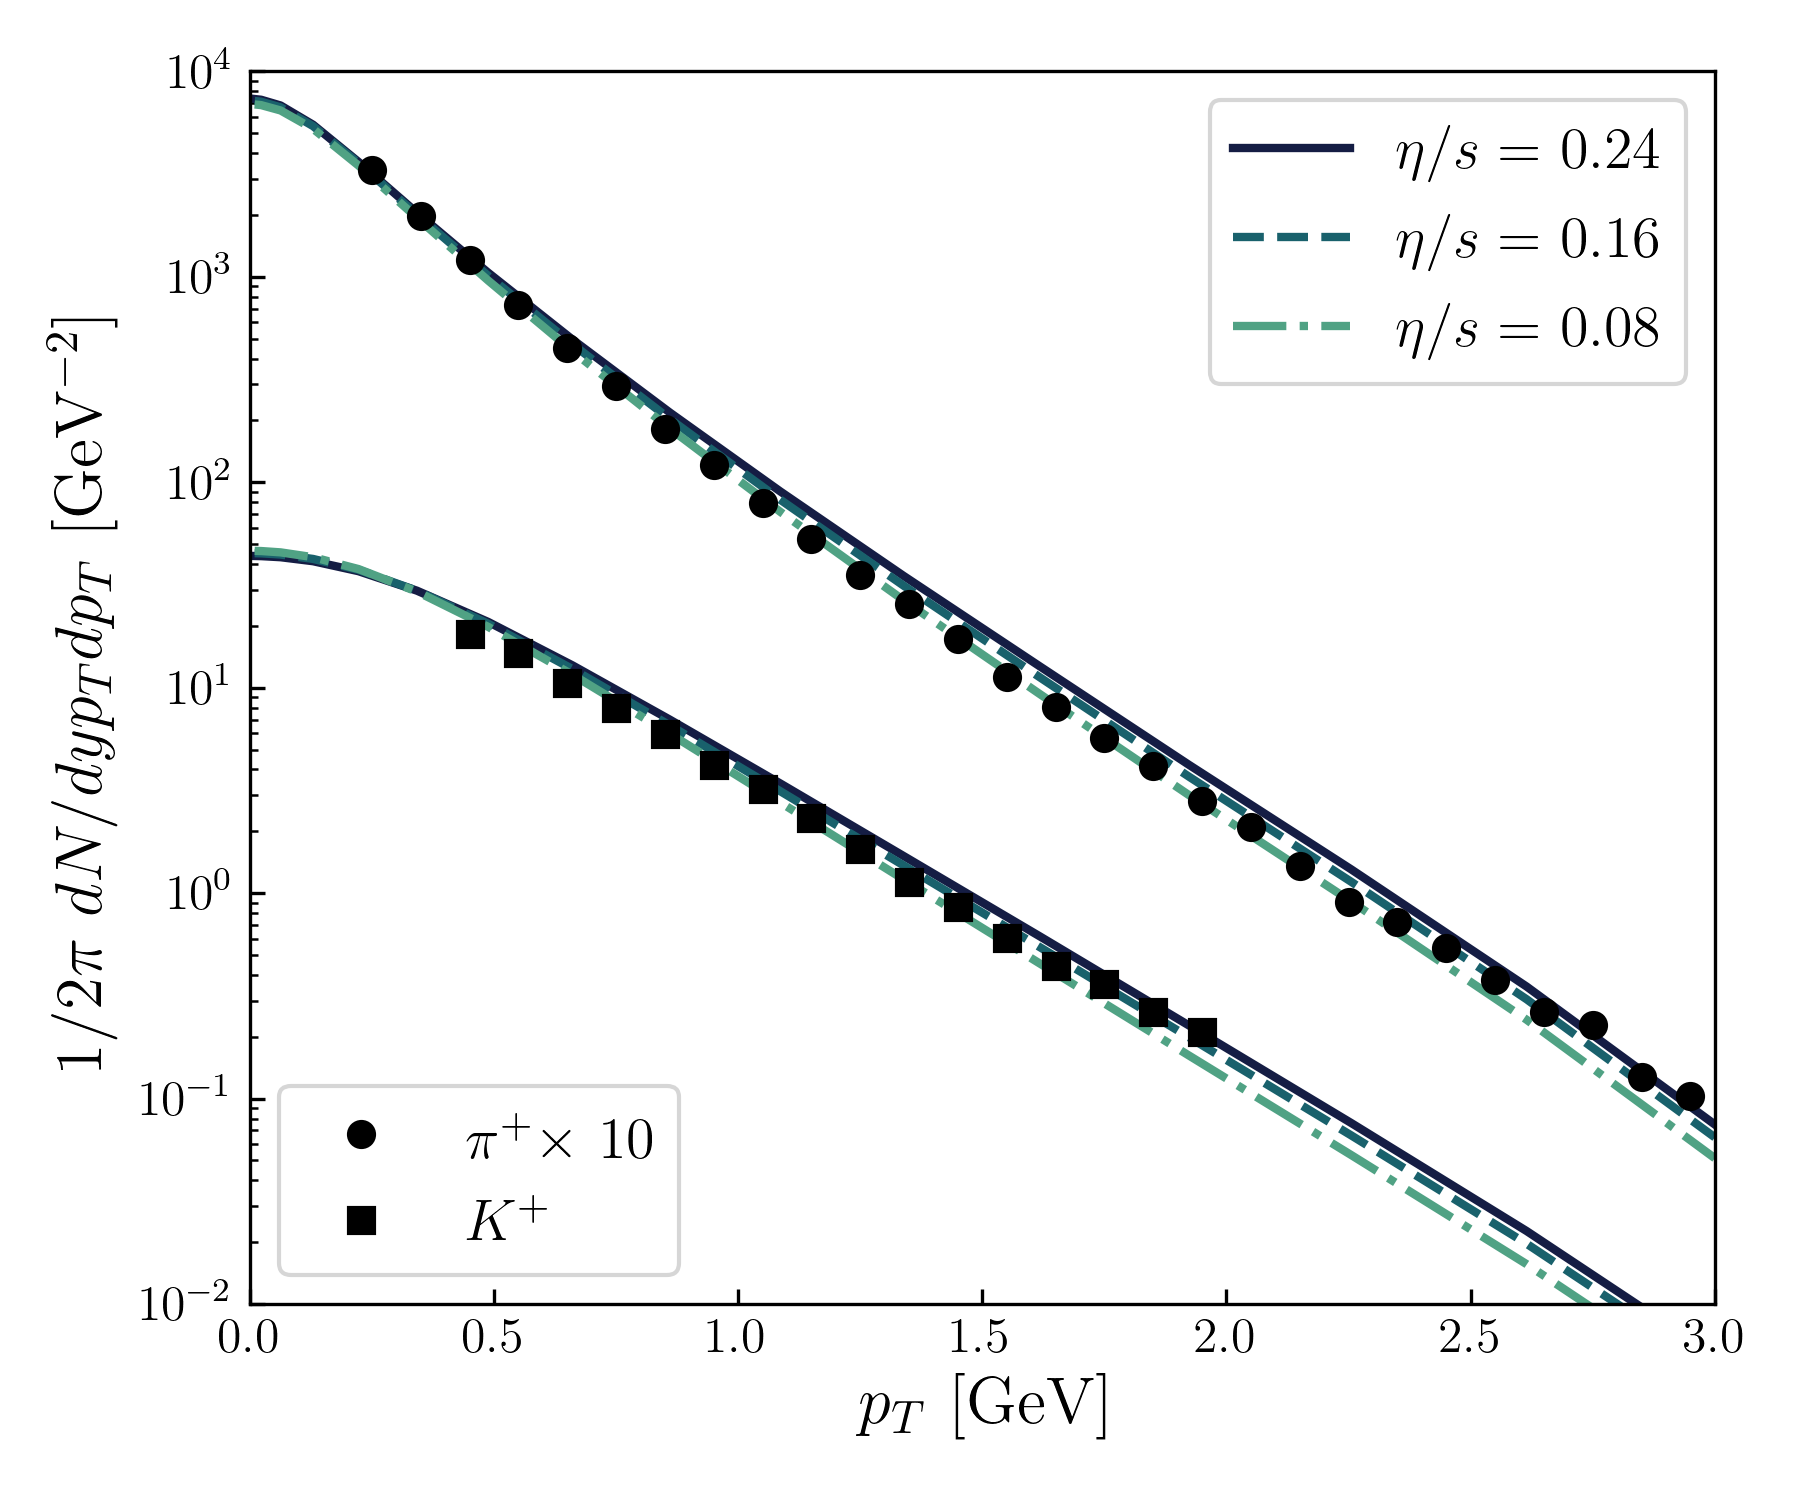
\includegraphics[width=\textwidth]{images/plot_etas_dep.png}
	\caption{\normalsize Transverse momentum spectra for positively charged pions and kaons of $0$-$5\%$ centrality, with fixed $s_\text{factor}=1.6$ and $T_\text{fo}=180$ MeV but varying $\eta/s$. The results are compared to {\sffamily PHENIX} data \cite{Adler:2003cb}. The shear viscosity correction $\delta f_\text{shear}$ is included. Increasing $\eta/s$ leads to flatter spectra.} 
\end{figure}

\vspace{-0.5cm}

\begin{figure}[H]
	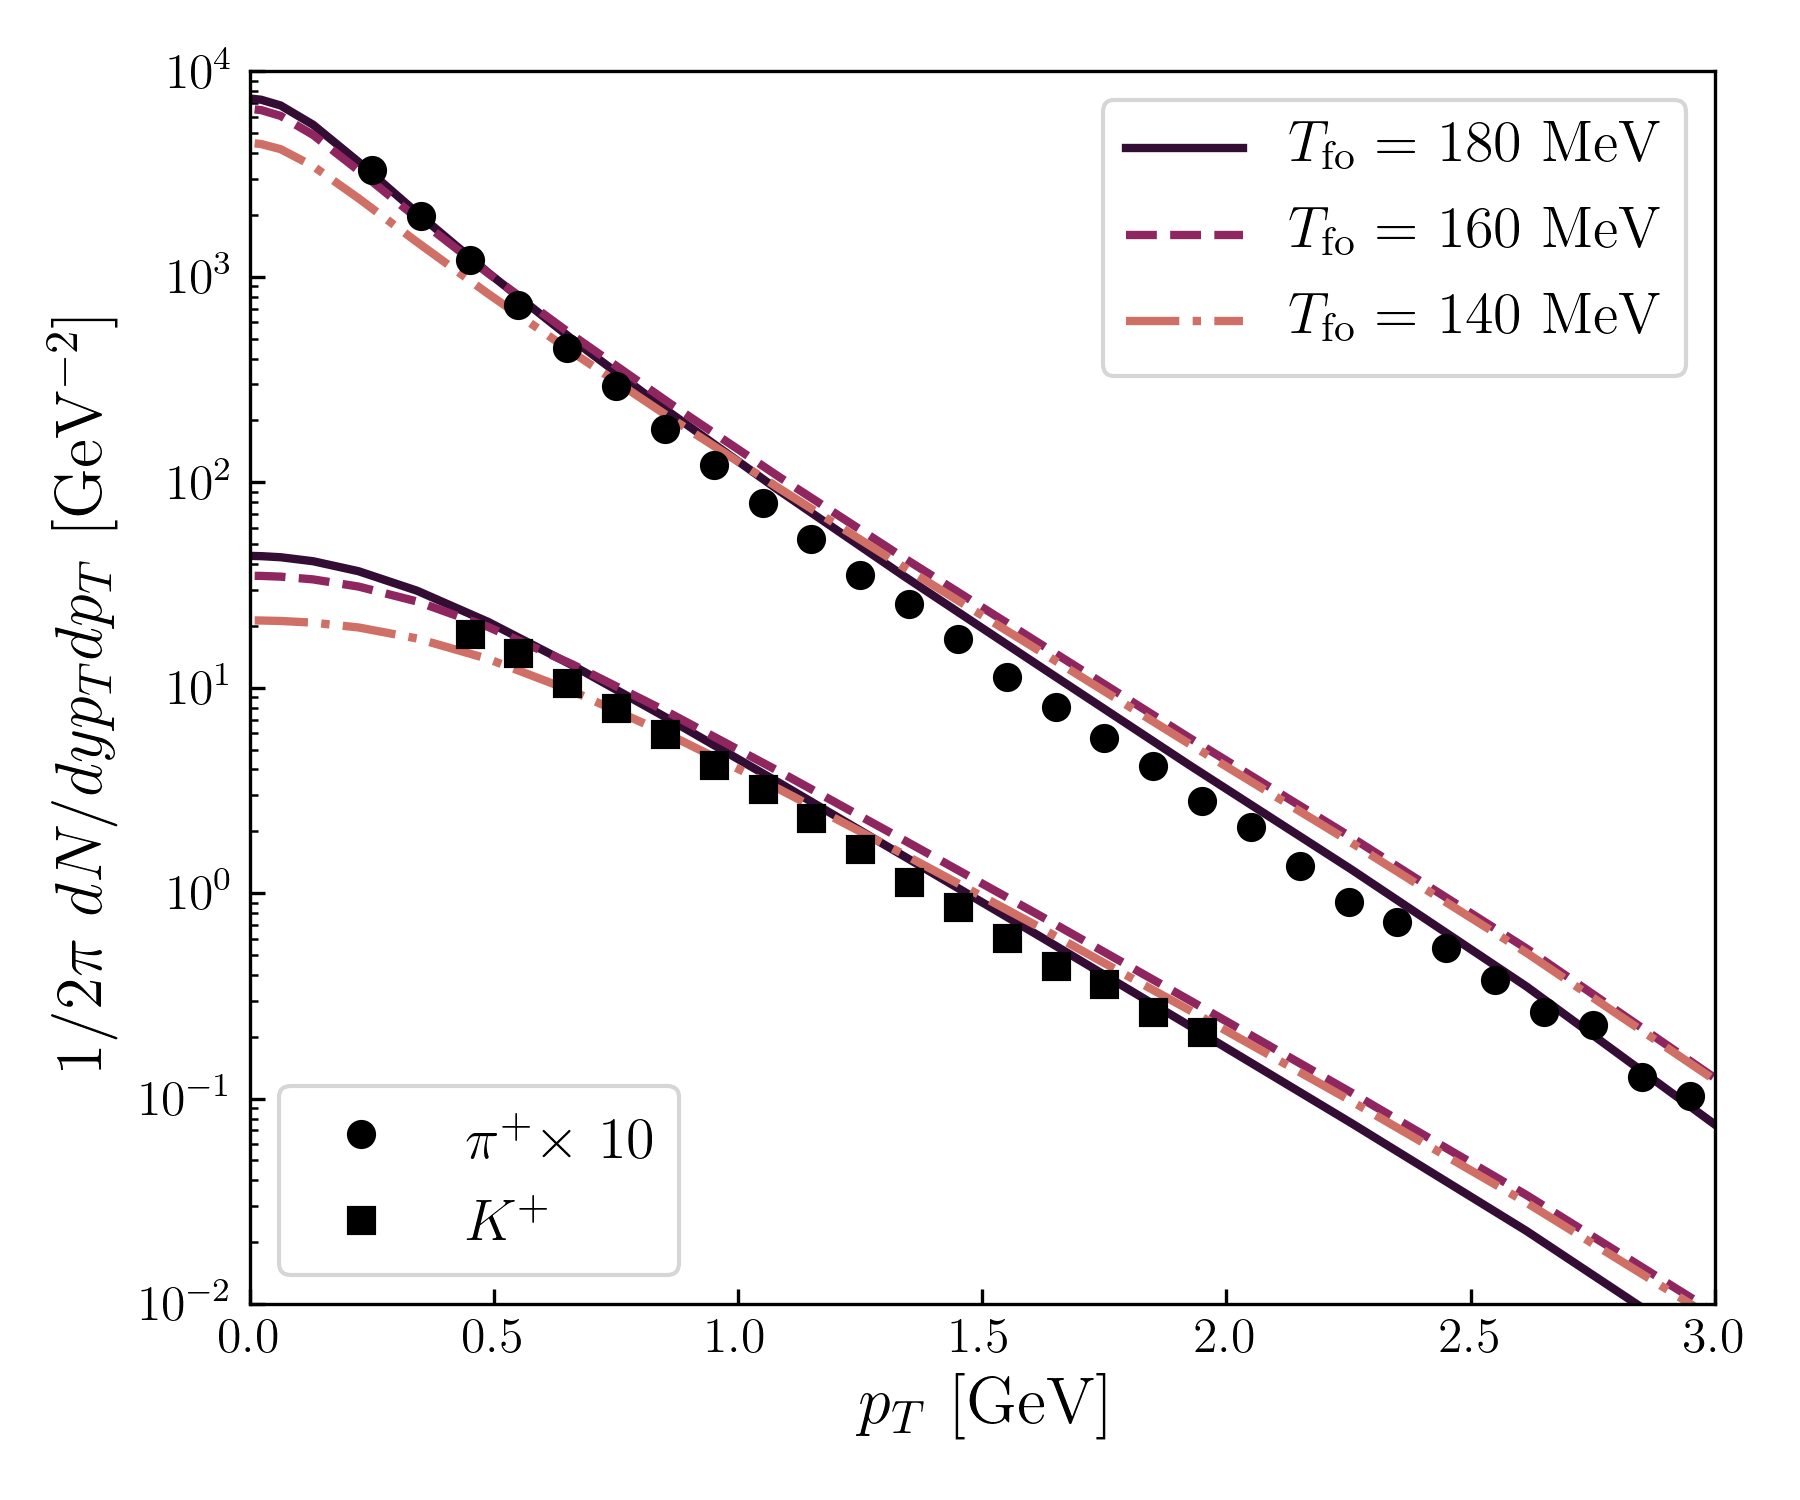
\includegraphics[width=\textwidth]{images/plot_tfo_dep.png}
	\caption{\normalsize Transverse momentum spectra for positively charged pions and kaons of $0$-$5\%$ centrality, with fixed $s_\text{factor}=1.6$ and $\eta/s=0.24$ MeV but varying $T_\text{fo}$. The results are compared to {\sffamily PHENIX} data \cite{Adler:2003cb}. The shear viscosity correction $\delta f_\text{shear}$ is included. Increasing $T_\text{fo}$ leads to steeper spectra.} 
\end{figure}

\begin{figure}[H]
	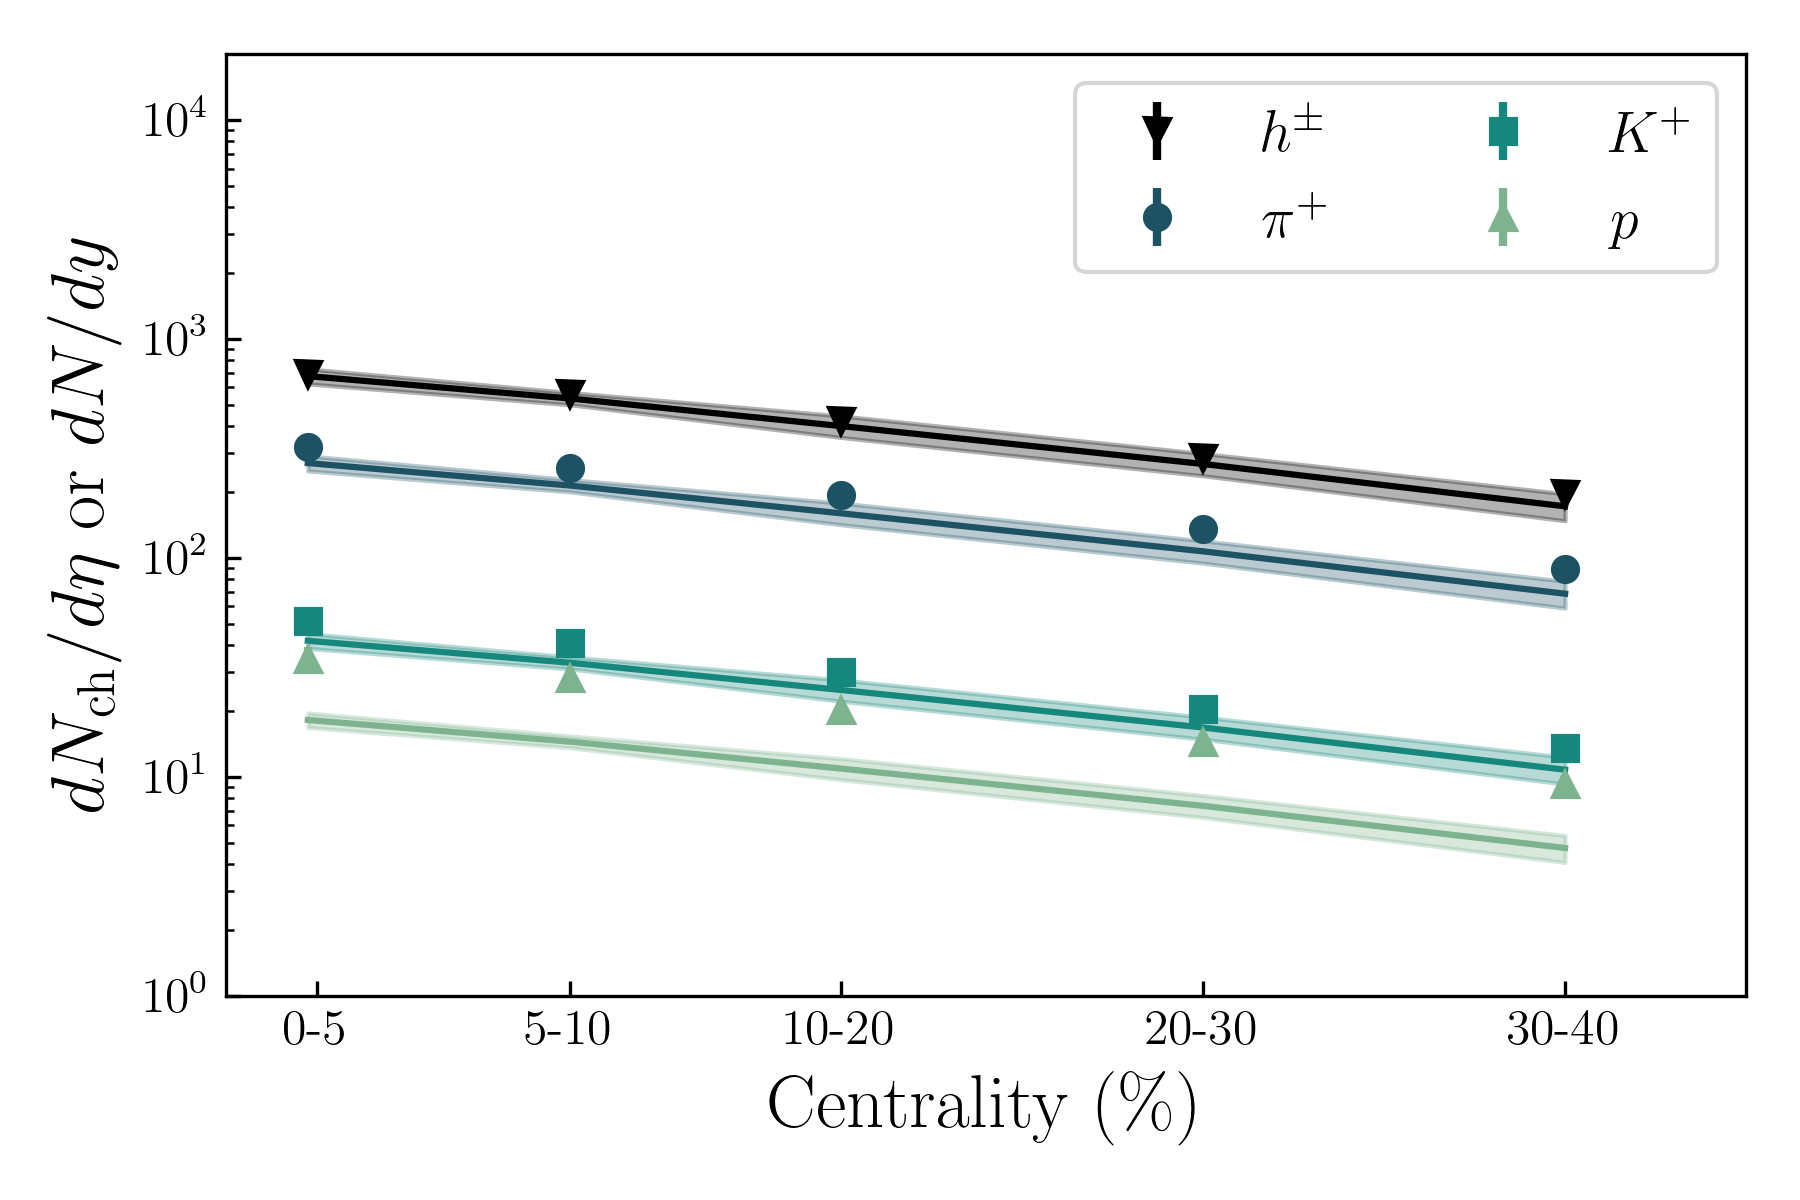
\includegraphics[width=\textwidth]{images/dn_cent_shear.png}
	\caption{\normalsize Charged particle multiplicity for all hadrons and positively charged pions, kaons and protons at different centralities. Data is taken from the tables provided in \cite{Abelev:2008ab}. The proton multiplicity is not well reproduced. In \cite{ryubulk} coupling {\sffamily MUSIC} to {\sffamily UrQMD} fixes this issue.} 
\end{figure}


\begin{figure}[H]
	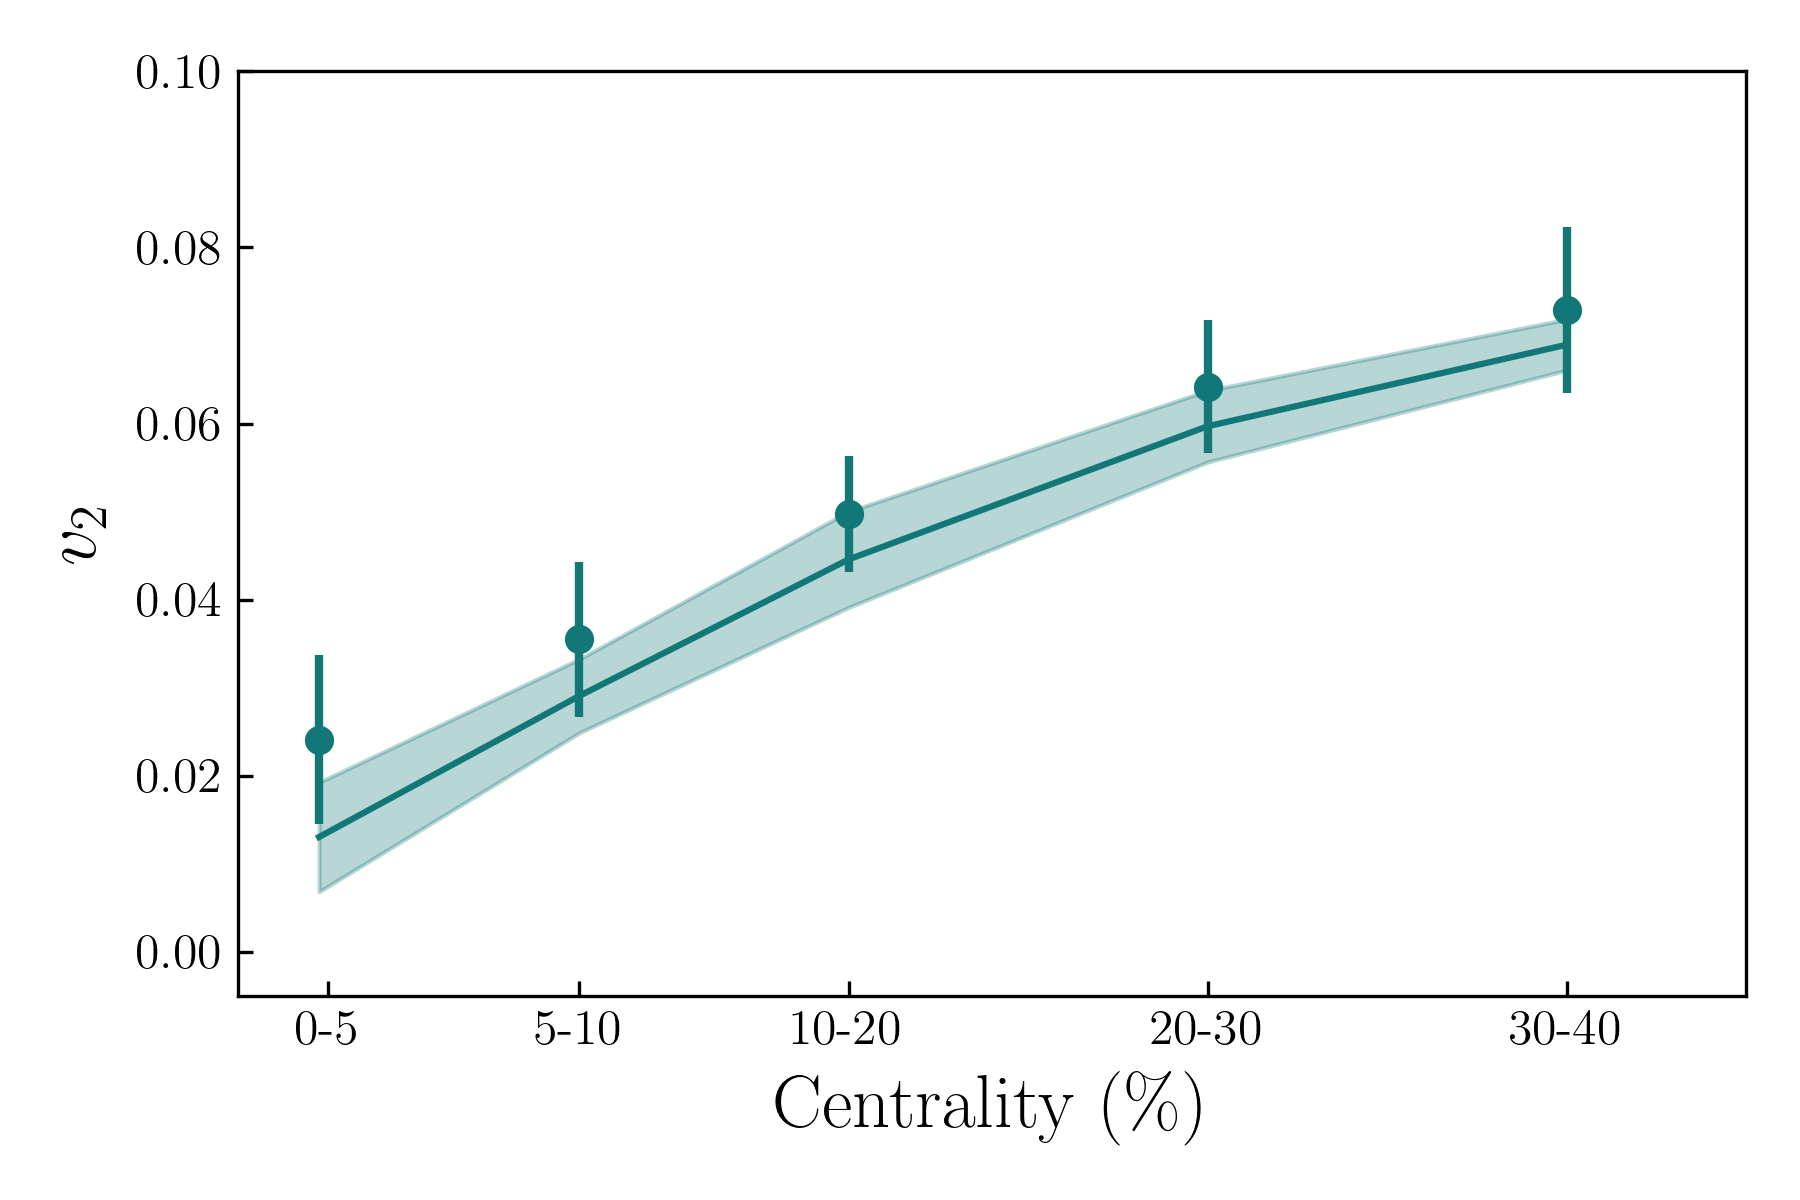
\includegraphics[width=\textwidth]{images/vn_cent.png}
	\caption{\normalsize Transverse momentum integrated elliptic flow of charged hadrons as a function of centrality. Data is taken from \cite{Abelev:2008ae}.} 
\end{figure}

\begin{figure}[H]
	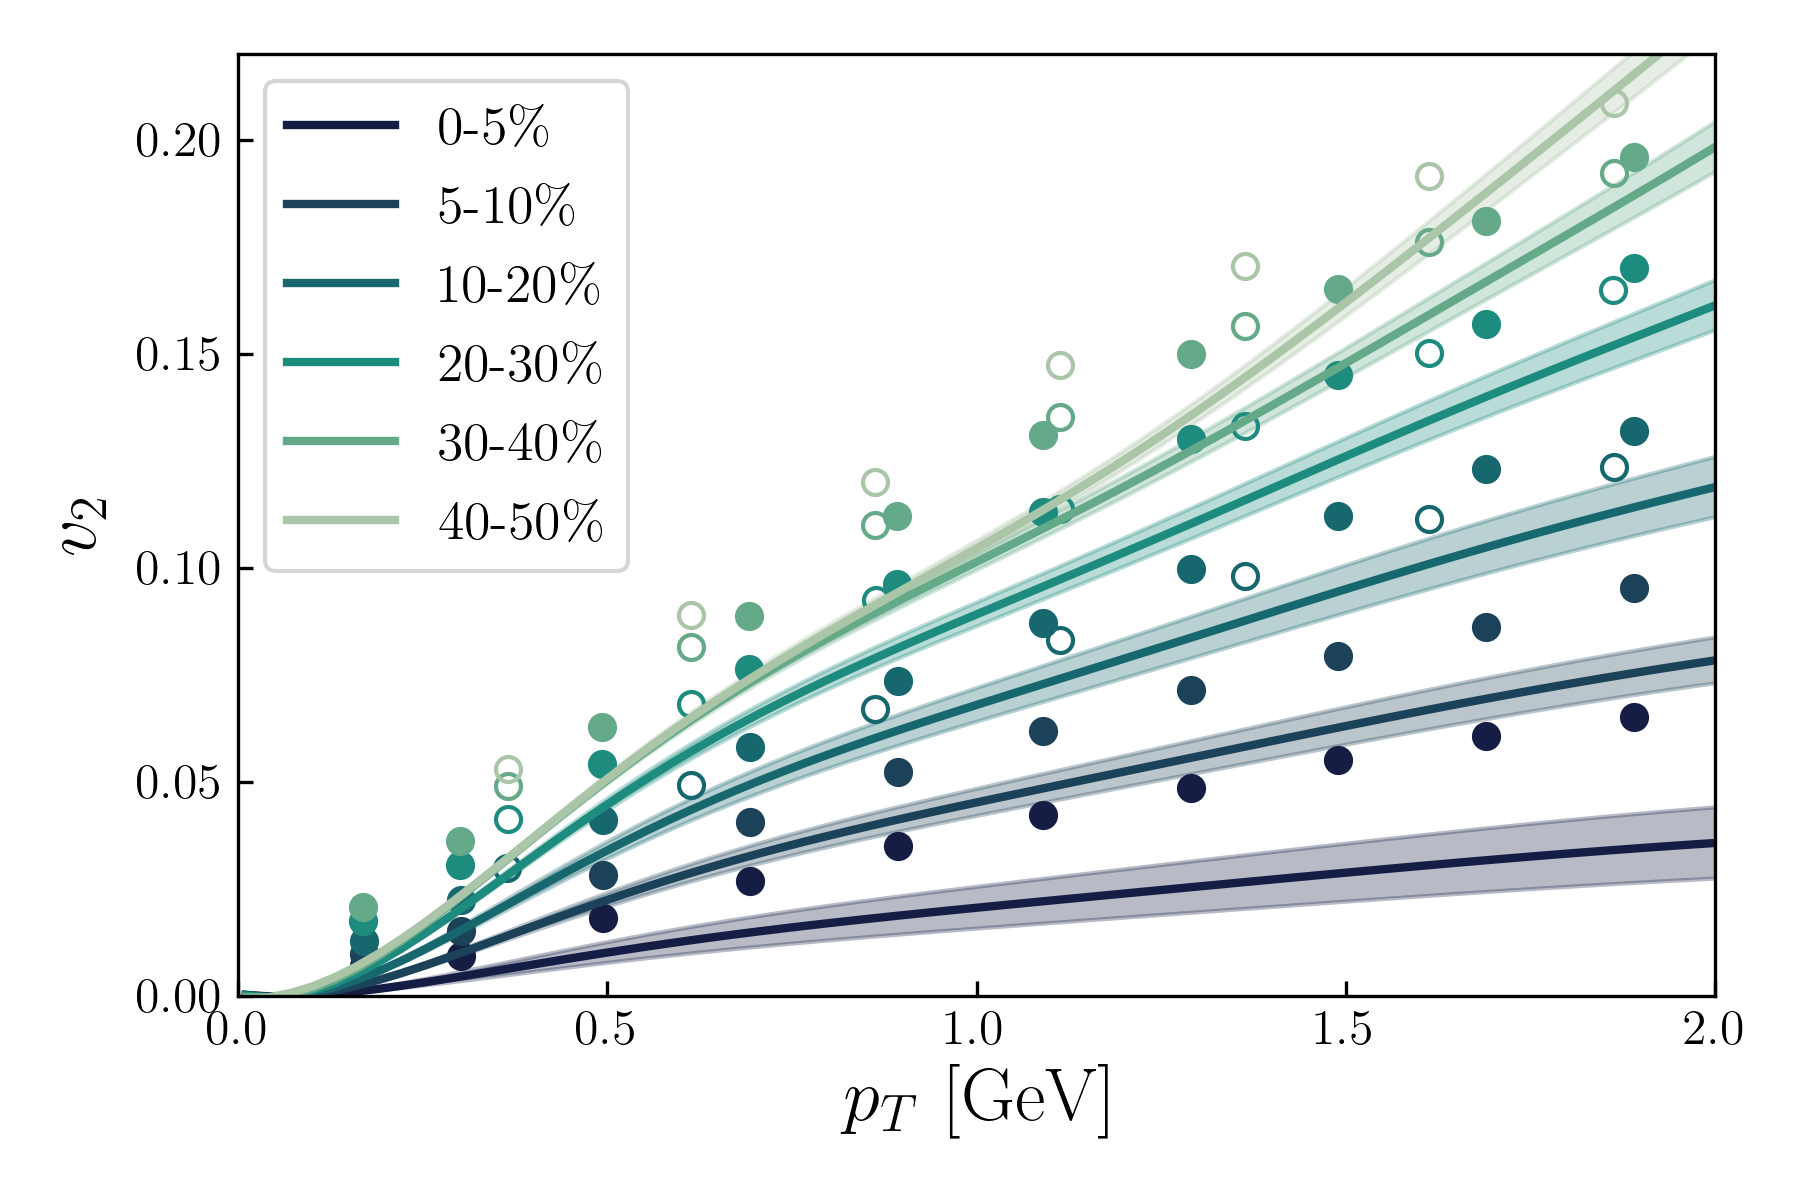
\includegraphics[width=\textwidth]{images/vn_pt.png}
	\caption{\normalsize Differential elliptic flow for charged hadrons at different centralities. The open symbols represent {\sffamily PHENIX} data points \cite{Adare:2011tg} whereas the filled correspond to {\sffamily STAR} data \cite{Adams:2004bi}.} 
\end{figure}

\begin{figure*}[!h]
	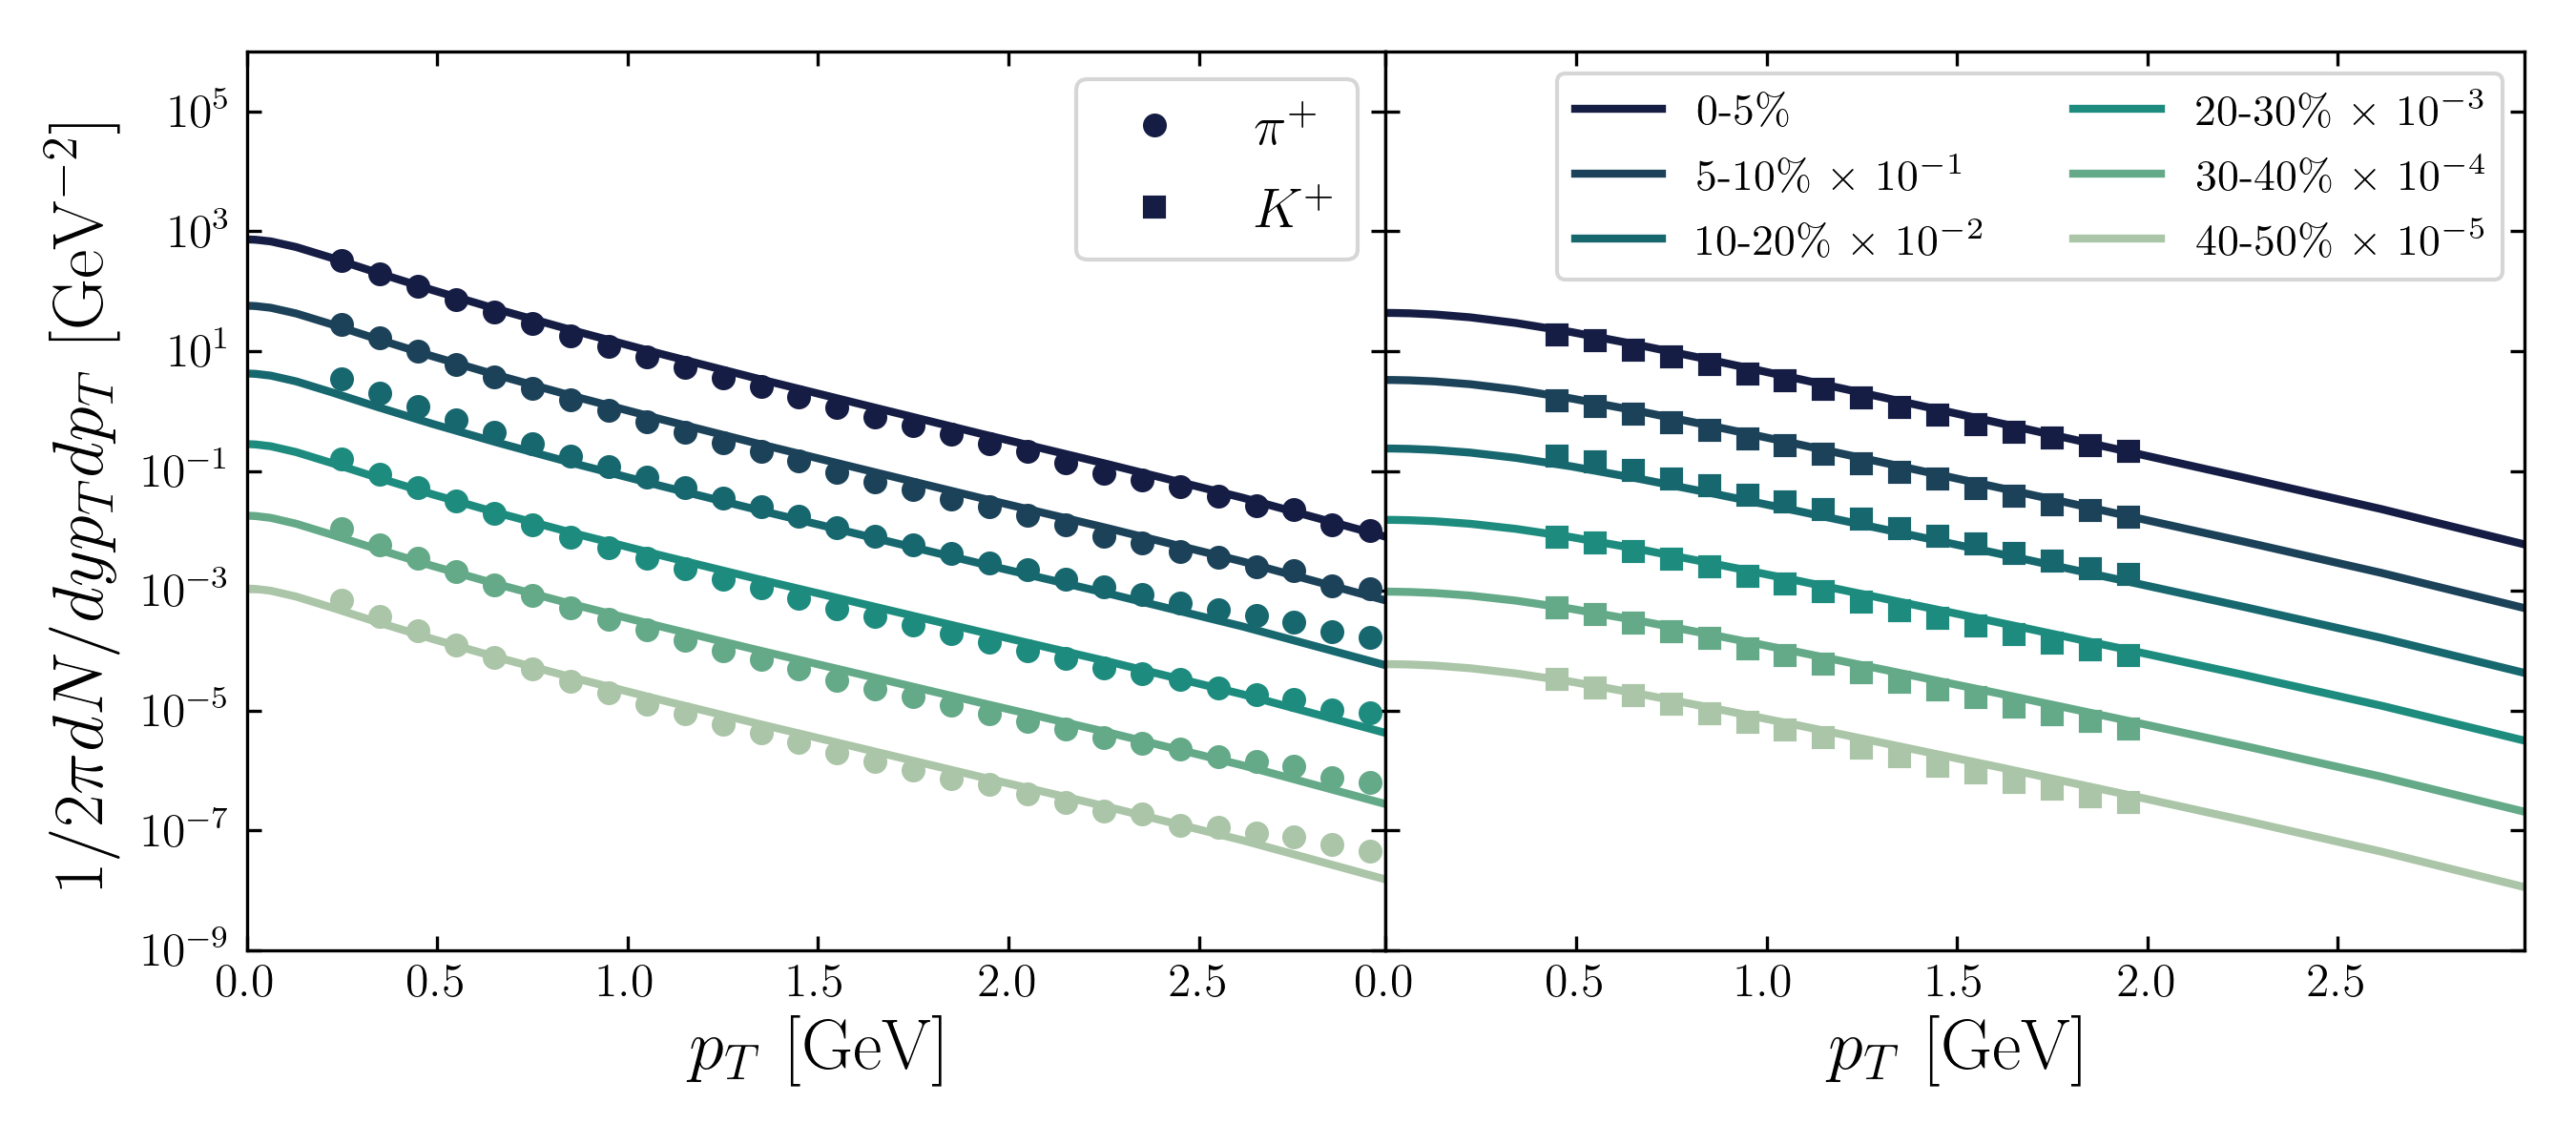
\includegraphics{images/plot_ptspectra_shear.png}
	\caption{\normalsize Transverse momentum spectra for positively charged pions and hadrons at different centralities. The results are compared to {\sffamily PHENIX} data \cite{Adler:2003cb}.}
\end{figure*}

\subsubsection*{Shear and bulk viscosities}
The minimal bayesian study described previously lead to the best fit parameters $s_\text{factor}=1.6$, $\eta/s=0.1$ and $T_\text{fo}=180$ MeV when bulk viscosity is also considered.

\begin{figure}[H]
    \figcolor{tealblue}
	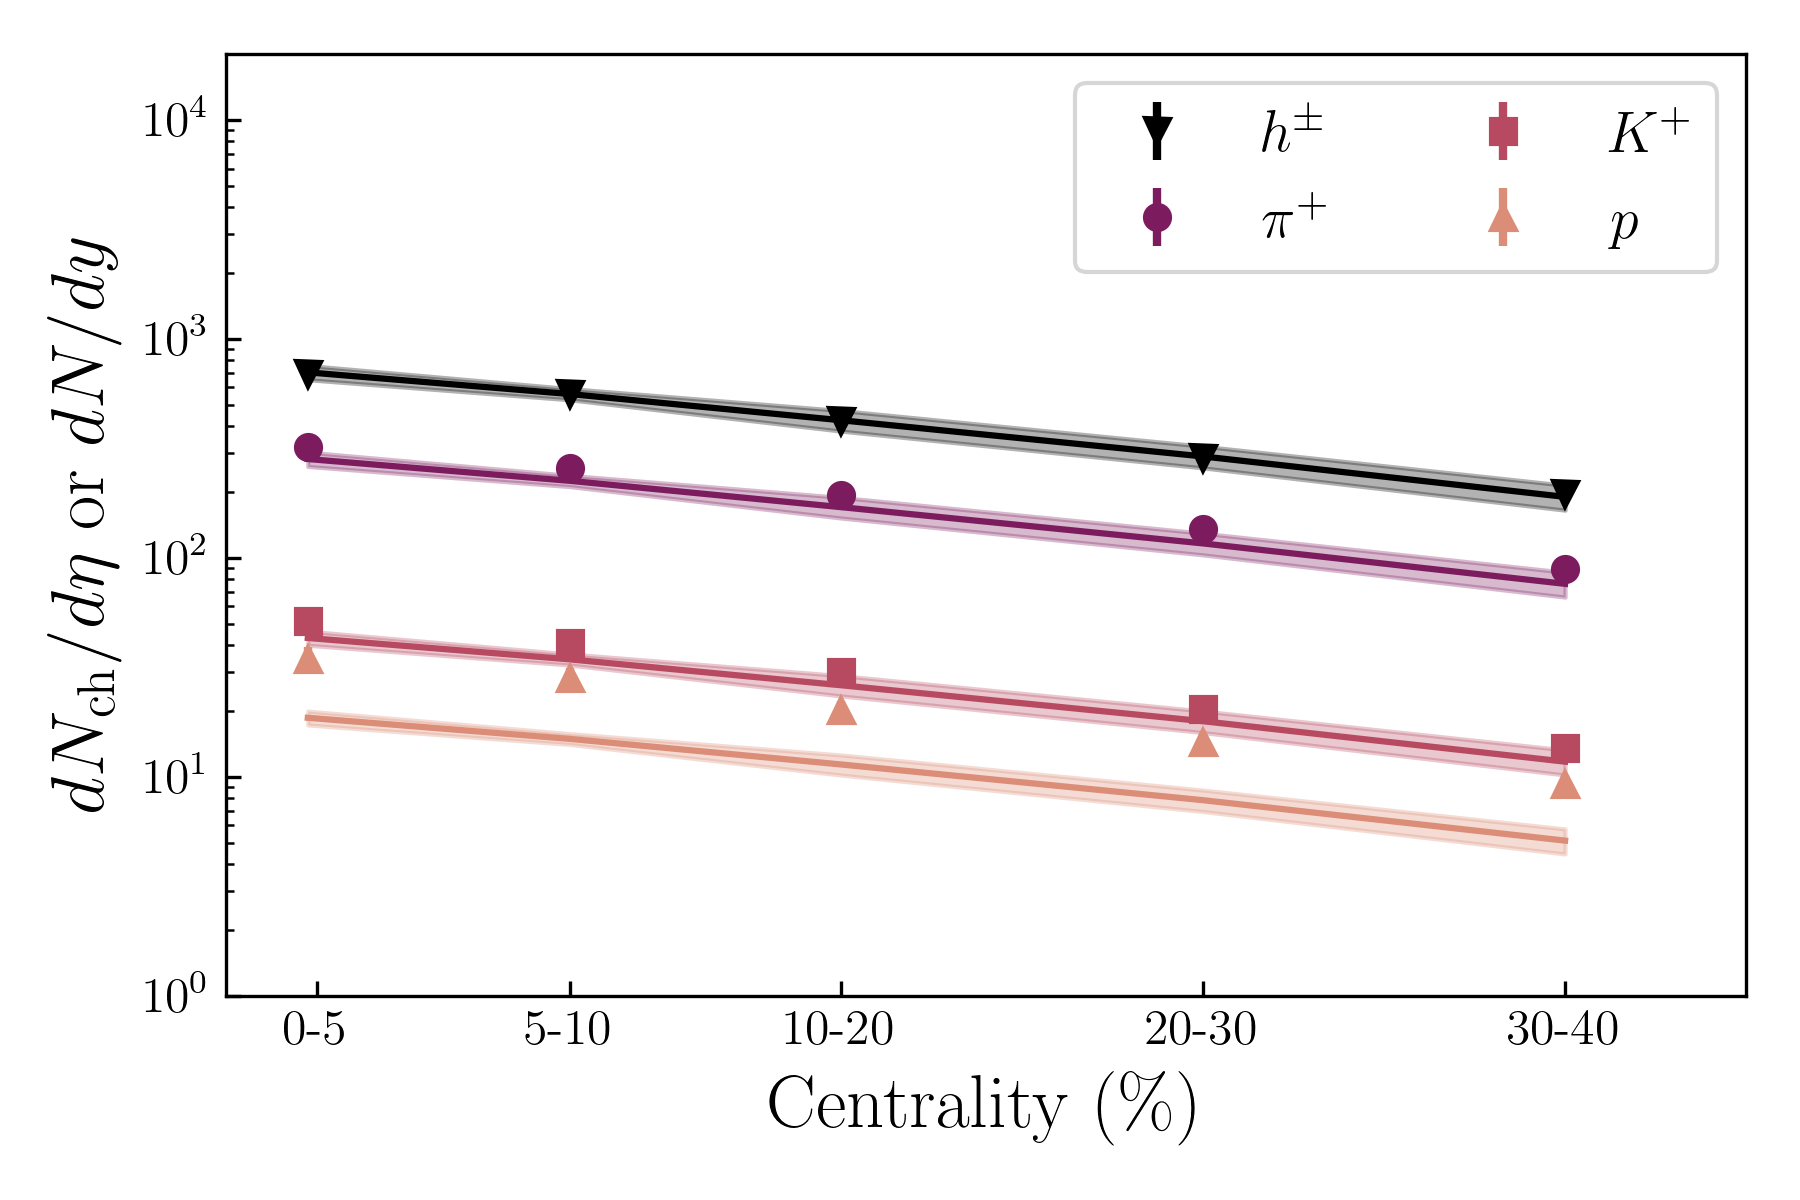
\includegraphics[width=\textwidth]{images/dn_cent_bulk.png}
	\caption{\normalsize Charged particle multiplicity for all hadrons and positively charged pions, kaons and protons at different centralities. Data is taken from the tables provided in \cite{Abelev:2008ab}. } 
\end{figure}

\begin{figure}[H]
    \figcolor{tealblue}
	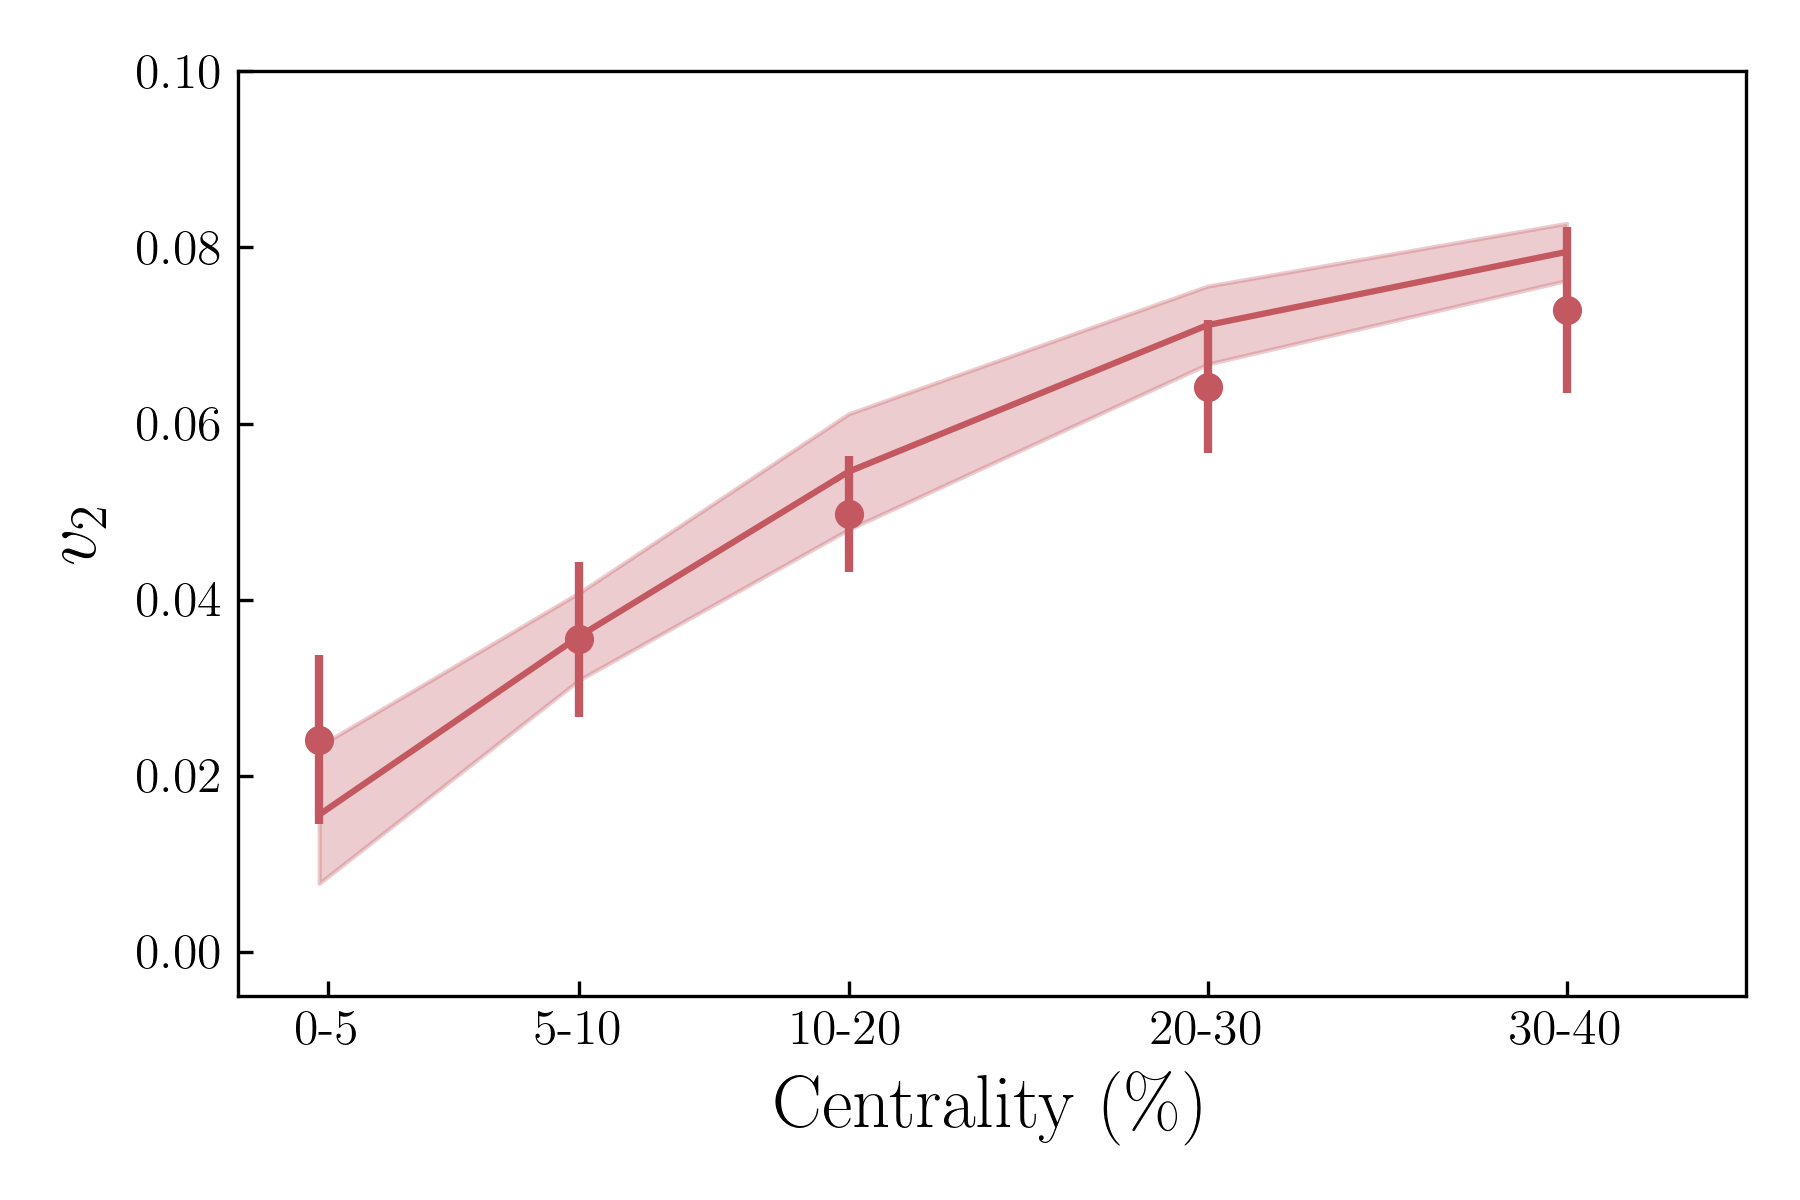
\includegraphics[width=\textwidth]{images/vn_cent_bulk.png}
	\caption{\normalsize Transverse momentum integrated elliptic flow of charged hadrons as a function of centrality. Data is taken from \cite{Abelev:2008ae}.} 
\end{figure}

\begin{figure*}[!h]
    \figcolor{tealblue}
	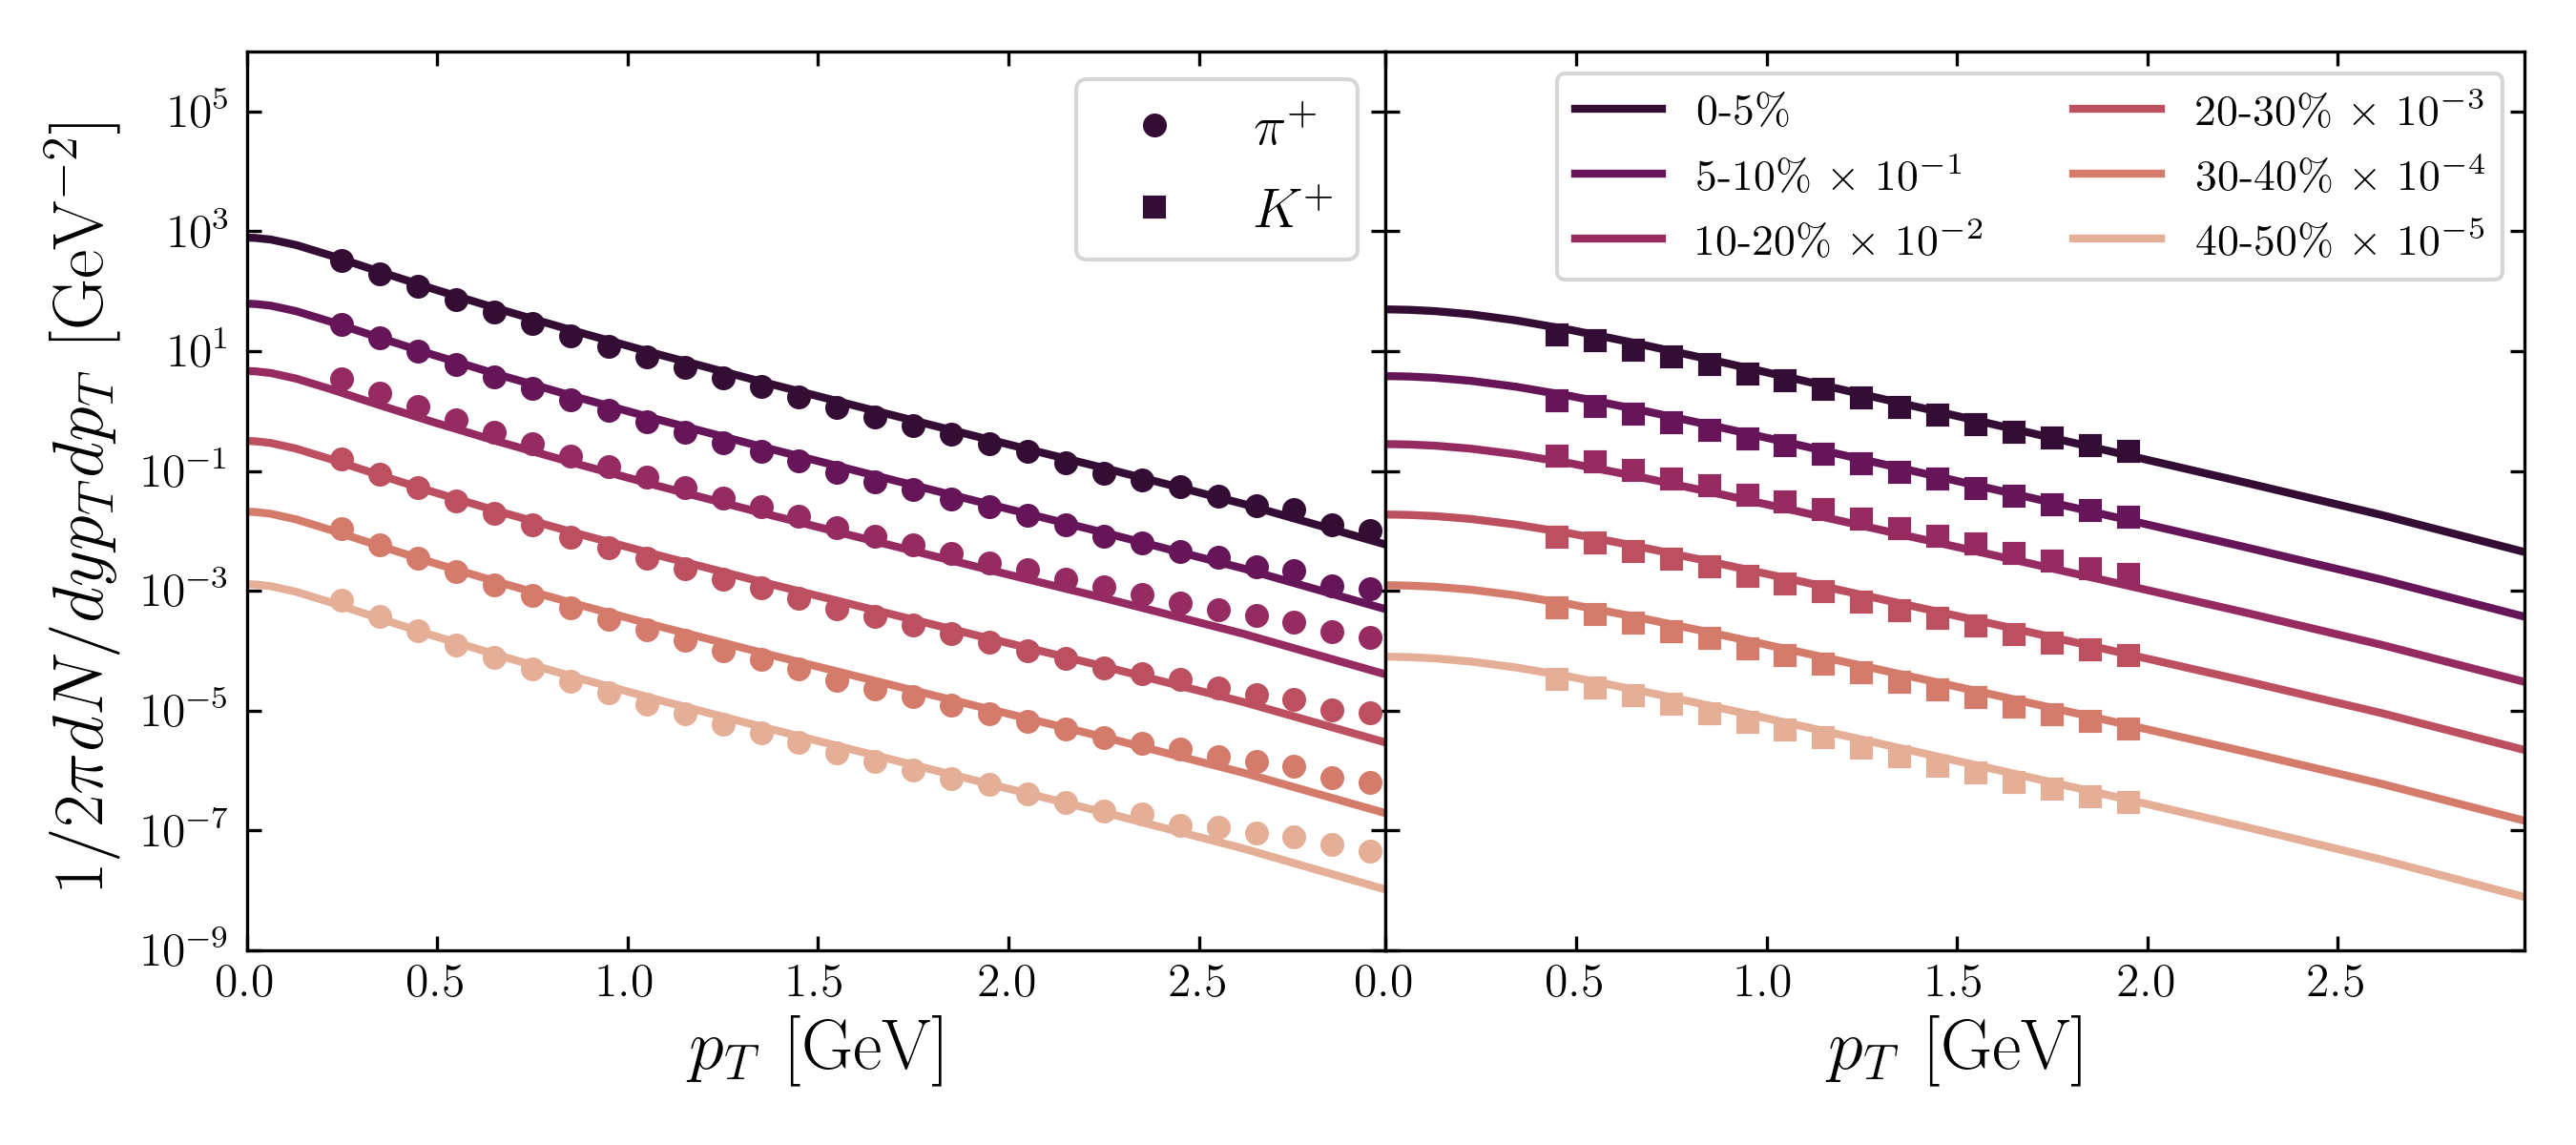
\includegraphics{images/plot_ptspectra_bulk.png}
	\caption{\normalsize Transverse momentum spectra for positively charged pions and hadrons at different centralities. The results are compared to {\sffamily PHENIX} data \cite{Adler:2003cb}.}
\end{figure*}

\begin{figure}[H]
    \figcolor{tealblue}
	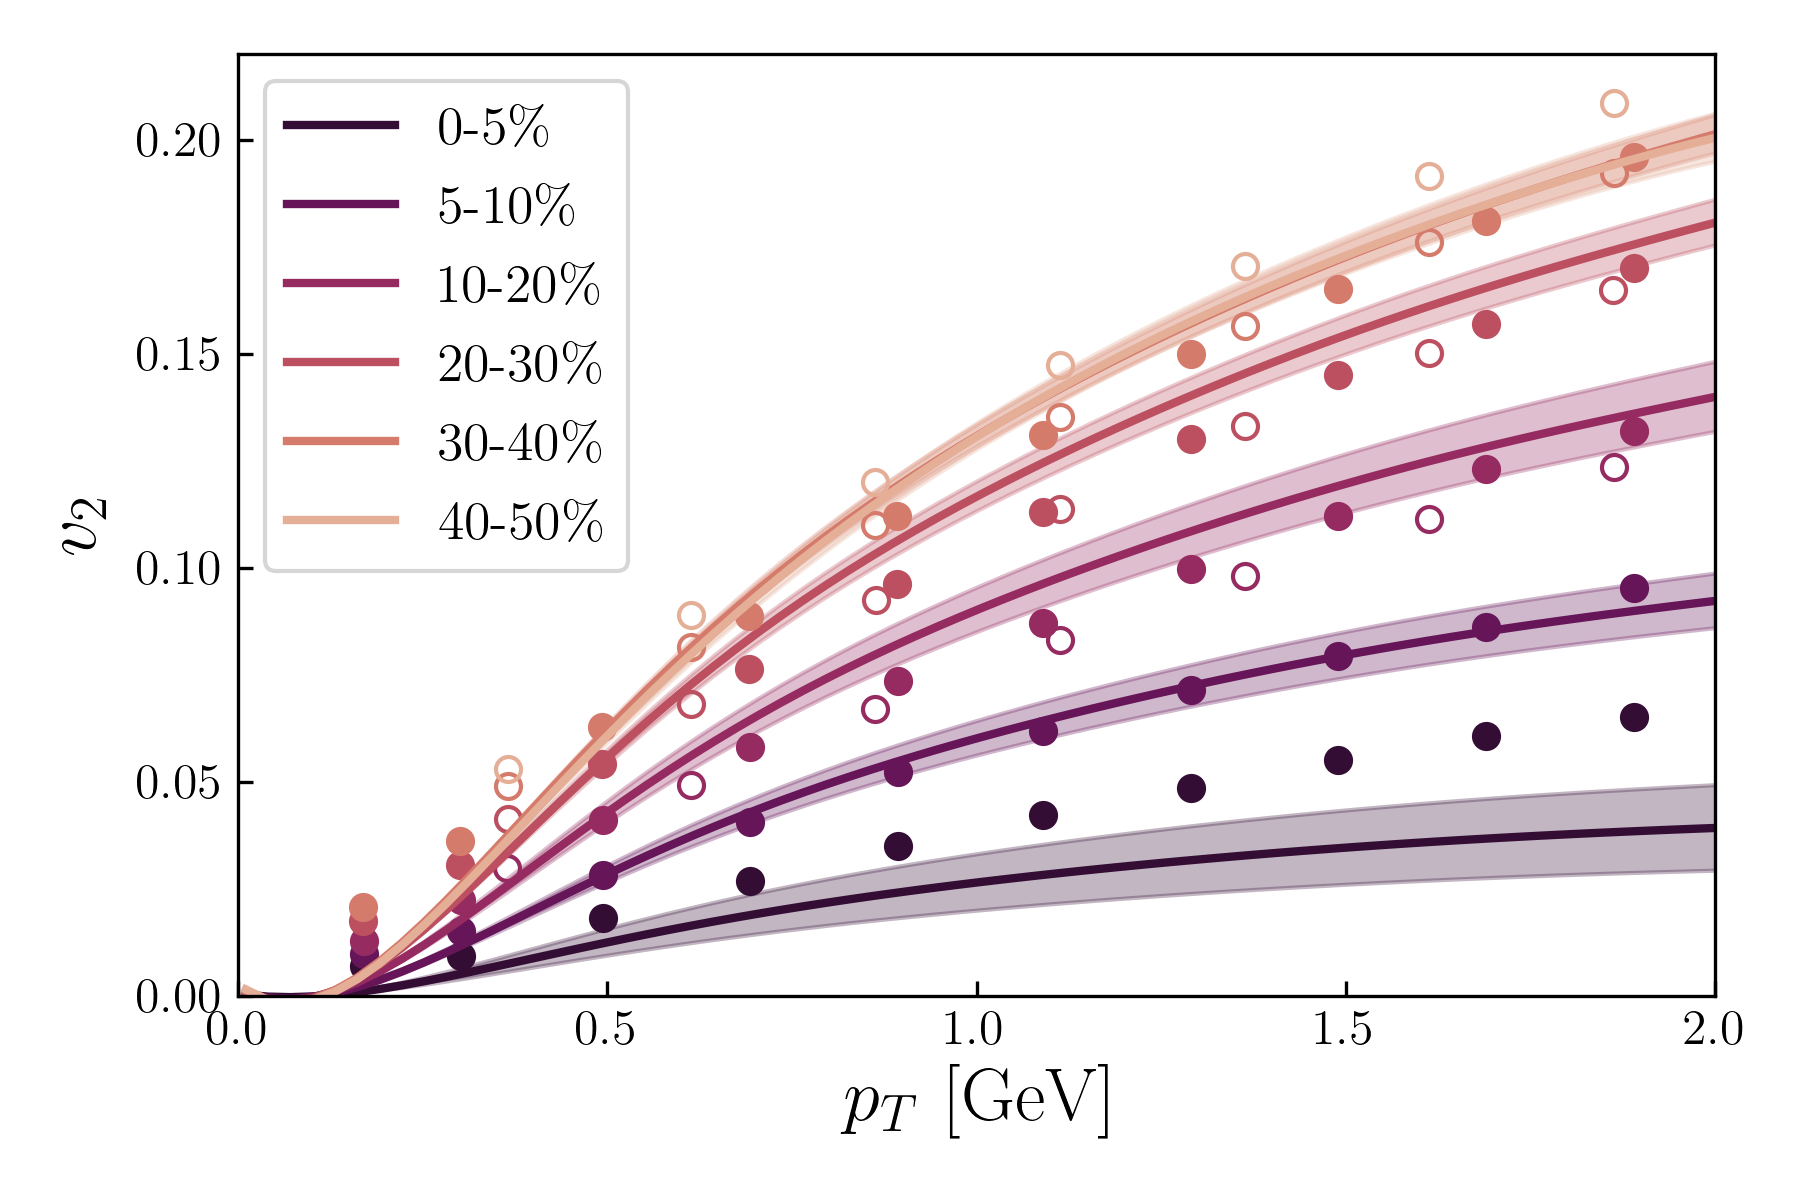
\includegraphics[width=\textwidth]{images/vn_pt_bulk.png}
	\caption{\normalsize Differential elliptic flow for charged hadrons at different centralities. The open symbols represent {\sffamily PHENIX} data points \cite{Adare:2011tg} whereas the filled correspond to {\sffamily STAR} data \cite{Adams:2004bi}.} 
\end{figure}

